\documentclass{article}

\def\npart{III}
\def\nyear{2018}
\def\nterm{Michaelmas}
\def\nlecturer{Professor W.\ T.\ Gowers}
\def\ncourse{Introduction to Discrete Analysis}
\def\draft{Rough, incomplete}
\usepackage{scalerel}
\usepackage{bbm}
\usepackage{mathdots}
\usepackage{chngcntr}
\usepackage{marginnote}
\ifx \nauthor\undefined
  \def\nauthor{Bhavik Mehta}
\else
\fi

\author{Based on lectures by \nlecturer \\\small Notes taken by \nauthor}
\date{\nterm\ \nyear}
\title{Part \npart\ -- \ncourse}

\usepackage[utf8]{inputenc}
\usepackage{amsmath}
\usepackage{amsthm}
\usepackage{amssymb}
\usepackage{enumerate}
\usepackage{mathtools}
\usepackage{graphicx}
\usepackage[dvipsnames]{xcolor}
\usepackage{tikz}
\usepackage{wrapfig}
\usepackage{centernot}
\usepackage{float}
\usepackage{braket}
\usepackage[hypcap=true]{caption}
\usepackage{enumitem}
\usepackage[colorlinks=true, linkcolor=mblue]{hyperref}
\usepackage[nameinlink,noabbrev]{cleveref}
\usepackage{nameref}
\usepackage[margin=1.5in]{geometry}

% Theorems
\theoremstyle{definition}
\newtheorem*{aim}{Aim}
\newtheorem*{axiom}{Axiom}
\newtheorem*{claim}{Claim}
\newtheorem*{cor}{Corollary}
\newtheorem*{conjecture}{Conjecture}
\newtheorem*{defi}{Definition}
\newtheorem*{eg}{Example}
\newtheorem*{ex}{Exercise}
\newtheorem*{fact}{Fact}
\newtheorem*{law}{Law}
\newtheorem*{lemma}{Lemma}
\newtheorem*{notation}{Notation}
\newtheorem*{prop}{Proposition}
\newtheorem*{question}{Question}
\newtheorem*{rrule}{Rule}
\newtheorem*{thm}{Theorem}
\newtheorem*{assumption}{Assumption}

\newtheorem*{remark}{Remark}
\newtheorem*{warning}{Warning}
\newtheorem*{exercise}{Exercise}

% \newcommand{\nthmautorefname}{Theorem}

\newtheorem{nthm}{Theorem}[section]
\newtheorem{nlemma}[nthm]{Lemma}
\newtheorem{nprop}[nthm]{Proposition}
\newtheorem{ncor}[nthm]{Corollary}
\newtheorem{ndef}[nthm]{Definition}

% Special sets
\newcommand{\C}{\mathbb{C}}
\newcommand{\N}{\mathbb{N}}
\newcommand{\Q}{\mathbb{Q}}
\newcommand{\R}{\mathbb{R}}
\newcommand{\Z}{\mathbb{Z}}

\newcommand{\abs}[1]{\left\lvert #1\right\rvert}
\newcommand{\norm}[1]{\left\lVert #1\right\rVert}
\renewcommand{\vec}[1]{\boldsymbol{\mathbf{#1}}}

\let\Im\relax
\let\Re\relax

\DeclareMathOperator{\Im}{Im}
\DeclareMathOperator{\Re}{Re}
\DeclareMathOperator{\id}{id}

\definecolor{mblue}{rgb}{0., 0.05, 0.6}


% https://tex.stackexchange.com/questions/100574/really-wide-hat-symbol
\usepackage{scalerel,stackengine}
\stackMath
\newcommand\reallywidehat[1]{%
\savestack{\tmpbox}{\stretchto{%
  \scaleto{%
    \scalerel*[\widthof{\ensuremath{#1}}]{\kern.1pt\mathchar"0362\kern.1pt}%
    {\rule{0ex}{\textheight}}%WIDTH-LIMITED CIRCUMFLEX
  }{\textheight}%
}{2.4ex}}%
\stackon[-6.9pt]{#1}{\tmpbox}%
}
\parskip 1ex

\usetikzlibrary{cd}
\reversemarginpar

\DeclareMathOperator*{\E}{\scalerel*{\mathbb{E}}{\textstyle\sum}}
\newcommand{\1}[1]{\mathbbm{1}_{#1}}
%\counterwithout{nthm}{section}
\DeclarePairedDelimiter\ceil{\lceil}{\rceil}
\DeclarePairedDelimiter\floor{\lfloor}{\rfloor}

\newcommand{\named}[1]{\textbf{#1}\index{#1}}

\DeclareMathOperator{\osc}{osc}
\DeclareMathOperator{\Var}{Var}
\DeclareMathOperator{\diam}{diam}

% preamble

%\setcounter{section}{-1}

% and here we go!

\begin{document}
\maketitle

\tableofcontents

\clearpage
\section{The Discrete Fourier transform}
Let $N$ be some fixed positive integer. Write $\omega$ for $e^{\frac{2\pi i}{N}}$, and $\mathbb{Z}_N$ for $\mathbb{Z}/N\mathbb{Z}$.

\begin{defi}[Discrete Fourier transform]\hypertarget{def:dft}
  Let $f: \mathbb{Z}_N \to \mathbb{C}$.
  Given $r \in \mathbb{Z}_N$, define $\hat{f}(r)$ to be
  \begin{equation*}
    \frac{1}{N} \sum_{x \in \mathbb{Z}_N} f(x) \omega^{-r x}.
  \end{equation*}
\end{defi}

\begin{notation}
  From now on, we shall use notation $\E_{x \in \mathbb{Z}_N}$ for $\frac{1}{N} \sum_{x \in \mathbb{Z}_N}$, where the subscript is omitted when it is clear from context.
\end{notation}

Notice we can write
\begin{equation*}
  \hat{f}(r) = \E_x f(x) e^{-\frac{2 \pi i r x}{N}},
\end{equation*}
highlighting the similarity with the usual Fourier transform.

% say something about cyclic groups and well-definedness?
If we write $\omega_r$ for the function $x \mapsto \omega^{r x}$, and $\langle f, g \rangle$ for $\E_x f(x) \overline{g(x)}$, then $\hat{f}(r) = \langle f, \omega_r \rangle$.
Let us write $\| f \|_p$ for $\left(\E_x |f(x)|^p\right)^{\frac{1}{p}}$ and call the resulting space $L_p(\mathbb{Z}_N)$.

\paragraph{Important convention.} We use \emph{averages} for the `original functions' in `physical space' and \emph{sums} for their Fourier transforms in `frequency space'.

% Lemma 1.
\begin{nlemma}[Parseval's identity]
  If $f,g: \mathbb{Z}_N \to \mathbb{C}$, then $\langle \hat{f}, \hat{g} \rangle = \langle f, g \rangle$.
\end{nlemma}
\begin{proof}
  \begin{align*}
    \langle \hat{f}, \hat{g} \rangle &= \sum_r \hat{f}(r) \overline{\hat{g}(r)} \\
                                     &= \sum_r (\E_x f(x) \omega^{-r x}) \overline{(\E_y g(y) \omega^{-r y})} \\
                                     &= \E_x \E_y f(x) \overline{g(y)} \sum_r \omega^{-r(x-y)} \\
                                     &= \E_x \E_y f(x) \overline{g(y)} \Delta_{xy} \\
                                     &= \E_x f(x) \E_y \overline{g(y)} \Delta_{xy} \\
                                     &= \E_x f(x) \overline{g(x)} = \langle f, g \rangle
  \end{align*}
  where
  \begin{equation*}
    \Delta_{xy} =
    \begin{cases}
      N & x = y \\
      0 & x \neq y.
    \end{cases} \qedhere
  \end{equation*}
   % reformat this...
\end{proof}

\begin{defi}[Convolution]\hypertarget{def:conv}
  The convolution $\widehat{f * g}(x)$ is defined to be \begin{equation*}\E_{y + z = x} f(y) g(z) = \E_y f(y) g(x-y).\end{equation*}
\end{defi}

\begin{nlemma}[Convolution identity]
  \begin{equation*}
    \widehat{\hyperlink{def:conv}{f * g}}(r) = \hat{f}(r) \hat{g}(r).
  \end{equation*}
\end{nlemma}
\begin{proof}
  \begin{align*}
    \widehat{f * g}(r) &= \E_x f * g(x) \omega^{-r x} \\
                       &= \E_x \E_{y + z = x} f(y) g(z) \omega^{- r x} \\
                       &= \E_x \E_{y + z = x} f(y) g(z) \omega^{- r y} \omega^{- r z} \\
                       &= \E_y f(y) \omega^{-r y} \E_z g(z) \omega^{-r z} = \hat{f}(r) \hat{g}(r). \qedhere
  \end{align*}
\end{proof}

\begin{nlemma}[Inversion formula]\label{lem:3}
  \begin{equation*}
    f(x) = \sum_r \hat{f}(r) \omega^{r x}
  \end{equation*}
\end{nlemma}
\begin{proof}
  \begin{align*}
    \sum_r \hat{f}(r) \omega^{r x} &= \sum_r \E_y f(y) \omega^{r (x-y)} \\
                                   &= \E_y f(y) \sum_r \omega^{r (x-y)} \\
                                   &= \E_y f(y) \Delta_{x y} = f(x). \qedhere
  \end{align*}
\end{proof}

Further observations:
\begin{itemize}
  \item If $f$ is real-valued, then $\hat{f}(-r) = \E_x f(x) \omega^{r x} = \overline{\E_x f(x) \omega^{- r x}} = \overline{\hat{f}(r)}$.
  \item If $A \subset \mathbb{Z}_n$, write $A$ (instead of $\1{A}$ or $\chi_A$) for the characteristic function of $A$.
    Then $\hat{A}(0) = \E_x A(x) = \frac{|A|}{N}$, the density of $A$.
  \item Also, $\|\hat{A}\|^2_2 = \langle \hat{A}, \hat{A} \rangle = \langle A, A \rangle = \E_x A(x)^2 = \E_x A(x) = \frac{A}{N}$.
\end{itemize}

Let $f : \mathbb{Z}_N \to \mathbb{C}$. Given $\mu \in \mathbb{Z}_N$ with $(\mu,N) = 1$, define $f_\mu(x)$ to be $f(\mu^{-1}x)$.
Then
\begin{align*}
  \hat{f_\mu}(r) &= \E_x f_\mu(x) \omega^{-r x} \\
                 &= \E_x f(x / \mu) \omega^{-r x}  \\
                 &= \E_x f(x) \omega^{- r \mu x}  \\
                 &= \hat{f}(\mu r).
\end{align*}

\subsection{Roth's Theorem}
\begin{nthm}\label{thm:1.4}
  For every $\delta > 0$, there exists $N$ such that if $A \subseteq \{1, \dotsc, N\}$ is a set of size at least $\delta N$ then $A$ must contain an arithmetic progression of length 3.
\end{nthm}
This is the $k=3$ case of Szemer\'{e}di's theorem.

Basic strategy: show that if $A$ has density $\geq \delta$ and no arithmetic progression of length 3, then there is a long arithmetic progression $P \subseteq \{1, \dotsc, N\}$ such that
\begin{equation*}
  |A \cap P| \geq (\delta + c(\delta)) |P|.
\end{equation*}
In particular, we have that $|P| \to \infty$ as $N \to \infty$.

The proof we give will produce a bound $\delta \geq \frac{C}{\log \log N}$, but this is not the best known.
If the bound was reduced to $\frac{1}{\log N}$, this produces a combinatorial proof of the fact that there are arbitrarily long arithmetic progressions in the primes.
The best known bound is $\frac{(\log \log N)^4}{\log N}$ by Thomas Bloom.
In the other direction, we know $e^{- \sqrt{\log N}}$ does not work.

% lecture 2
\begin{nlemma}\label{lem:1.5}
  Let $A, B, C \subset \mathbb{Z}_N$ have densities $\alpha, \beta, \gamma$, for $N$ odd.
  If $\max_{r \neq 0} |\hat{A}(r)| \leq \frac{\alpha(\beta \gamma)^\frac{1}{2}}{2}$ and $\frac{\alpha\beta\gamma}{2} > \frac{1}{N}$ then there exists $x,d \in \mathbb{Z}_N$ with $d \neq 0$ such that $(x, x+d, x+2d) \in A \times B \times C$.
\end{nlemma}
\begin{proof}
  \begin{align*}
    \E_{x,d} A(x) B(x+d) C(x+2d) &= \E_{\mathclap{x + z = 2y}} A(x) B(y) C(z) \\
                                 &= \E_u (\E_{x+z=u} A(x) C(z)) \E_{2y=u} B(y) \\
                                 &= \E_u (A * C)(u) B_2(u) = \langle A * C, B_2 \rangle \\
                                 &= \langle \widehat{A * C}, \hat{B} _2 \rangle \\
                                 &= \langle \hat{A} \hat{C}, \hat{B}_2 \rangle \\
                                 &= \sum_r \hat{A}(r) \hat{C}(r) \hat{B}(-2r) \\
                                 &= \alpha \beta \gamma + \sum_{r\neq 0} \hat{A}(r) \hat{C}(r) \hat{B}(-2r).
  \end{align*}
  We have a lower bound on the left term, so focus on the right.
  \begin{align*}
    \left| \sum_{r\neq0} \hat{A}(r) \hat{B}(-2r) \hat{C}(r) \right| &\leq \frac{\alpha(\beta\gamma)^\frac{1}{2}}{2} \sum_{r\neq0} |\hat{B}(-2r) \hat{C}(r)| \\
                                                      &\leq \frac{\alpha(\beta\gamma)^\frac{1}{2}}{2} \left(\sum_r |\hat{B}(-2r)|^2\right)^\frac{1}{2} \left(\sum_r |\hat{C}(r)|^2\right)^\frac{1}{2} \\
                                                      &= \frac{\alpha(\beta\gamma)^\frac{1}{2}}{2} \|\hat{B}\|_2 \|\hat{C}\|_2 = \frac{\alpha(\beta\gamma)^\frac{1}{2}}{2} \|B\|_2 \|C\|_2 \\
                                                      &= \frac{\alpha\beta\gamma}{2}.
  \end{align*}
  The contribution to $\E_{x,d} A(x) B(x+d) C(x+2d)$ from $d=0$ is at most $\frac{1}{N}$, so if $\frac{\alpha\beta\gamma}{2} > \frac{1}{N}$, we are done.
\end{proof}

Now let $A$ be a subset of $\{1, \dotsc, N\}$ of density $\geq \delta$ and let $B = C = A \cap (\frac{N}{3}, \frac{2N}{3}]$.
If $B$ has density $< \frac{\delta}{5}$, then either $A \cap [1, \frac{N}{3}]$ or $A \cap [\frac{2N}{3}, N]$ has density at least $\frac{2 \delta}{5}$.
So in that case we find an AP $P$ of length about $\frac{N}{3}$ such that $\frac{|A \cap P|}{|P|} \geq \frac{6 \delta}{5}$.

Otherwise, we find that if $\max_{r \neq 0} |\hat{A}(r)| \leq \frac{\delta^2}{10}$ and $\frac{\delta^3}{50} > \frac{1}{N}$ then $A \times B \times C$ contains a 3AP $\implies A$ contains a 3AP.
So if $A$ does not contain a 3AP, then either we find $P$ of length about $\frac{N}{3}$ with $\frac{|A \cap P|}{|P|} \geq \frac{6 \delta}{5}$ or $\exists r \neq 0$ such that $|\hat{A}(r)| \geq \frac{\delta^2}{10}$.

\begin{defi}
  If $X$ is a finite set and $f: X \to \mathbb{C}$, $Y \subseteq X$, write $\osc(f|_Y)$ to mean $\max_{y_1, y_2 \in Y} |f(y_1) - f(y_2)|$.
\end{defi}
\begin{nlemma}\label{lem:1.6}
  Let $r \in \hat{\mathbb{Z}}_n$ and let $\epsilon > 0$. Then there is a partition of $\{1,2,\dotsc,N\}$ into arithmetic progressions $P_i$ of length at least $c(\epsilon) \sqrt{N}$ such that $\osc(\omega_r|_{P_i}) \leq \epsilon$ for each $i$.
\end{nlemma}
\begin{proof}
  Let $t = \floor{\sqrt{N}}$. Of the numbers $1, \omega^r, \omega^{2r}, \dotsc, \omega^{tr}$ there must be two that differ by at most $\frac{2\pi}{t}$.
  If $|\omega^{ar} - \omega^{br}| \leq \frac{2\pi}{t}$ with $a < b$, then $|1 - \omega^{dr}| \leq \frac{2\pi}{t}$ where $d = b-a$.
  Now, by the triangle inequality, if $u < v$, then
  \begin{equation*}
    |\omega^{u rd} - \omega^{v r d}| \leq |\omega^{urd} - \omega^{(u+1) r d}| + |\omega^{urd} - \omega^{(u+1) r d}| + \dotsb + |\omega^{urd} - \omega^{(u+1) r d}| \leq \frac{2\pi}{t} (v-u).
  \end{equation*}
  So if $P$ is a progression with common difference $d$ and length $l$, then $\osc(\omega_r|_P) \leq \frac{2\pi l}{t}$.
  So divide up $\{1,\dotsc,N\}$ into residue classes mod $d$ and partition each residue class into parts of length between $\frac{\epsilon t}{4 \pi}$ and $\frac{\epsilon t}{2 \pi}$ (possible, since $d \leq t \leq \sqrt{N}$).
  We are done, with $c(\epsilon) = \frac{\epsilon}{16}$.
\end{proof}
Now let us use the information that $r \neq 0$ and $|\hat{A}(r)| \geq \frac{\delta^2}{10}$.
Define the balanced function $f$ of $A$ by $f(x) = A(x) - \frac{|A|}{N}$ for each $x$.

Note that $\hat{f}(0) = 0$ and $\hat{f}(r) = \hat{A}(r)$ for all $r \neq 0$.
Now let $P_1, \dotsc, P_m$ be given by \cref{lem:1.6} with $\epsilon = \frac{\delta^2}{20}$.
Then
\begin{align*}
  \frac{\delta^2}{10} \leq \frac{1}{N} \left| \sum_x f(x) \omega^{-rx} \right| &\leq \frac{1}{N} \sum_{i=1}^m \left|\sum_{x\in P_i} f(x) \omega^{-r x}\right| \\
                                                                      &\leq \frac{1}{N} \sum_{i=1}^m \left[\left|\sum_{x \in P_i} f(x) \omega^{-r x_i}\right| + \left|\sum_{x \in P_i} f(x) (\omega^{-r x} - \omega^{-r x_i})\right|\right] \\
                                                                      \shortintertext{where $x_i \in P_i$ is arbitrary }
                                                                      &\leq \frac{1}{N} \sum_{i=1}^m \left|\sum_{x \in P_i} f(x)\right| + \frac{\delta^2}{20}
                                                                      \shortintertext{So}
  \sum_{i=1}^N \left|\sum_{x \in P_i} f(x) \right| &\geq \frac{\delta^2 N}{20}.
\end{align*}
Also,
\begin{equation*}
  \sum_{i=1}^m \sum_{x \in P_i} f(x) = 0.
\end{equation*}
So
\begin{equation*}
  \sum_{i=1} \left( \left|\sum_{x \in P_i} f(x) \right| + \sum_{x \in P_i} f(x) \right)  \geq \frac{\delta^2}{20}  \sum_{i =1}^m |P_i|
\end{equation*}
Therefore, $\exists i$ such that
\begin{align*}
  \left| \sum_{x \in P_i} f(x) \right| + \sum_{x \in P_i} f(x) &\geq \frac{\delta^2}{20} |P_i| \\
  \implies \sum_{x \in P_i} f(x) \geq \frac{\delta}{40} |P_i| \\
  \implies |A \cap P_i| \geq \left(\delta + \frac{\delta^2}{40}\right) |P_i|
\end{align*}

% lecture 3
So now, either
\begin{enumerate}
  \item $A$ contains a $3AP$
  \item $N$ is even
  \item $\exists P \subset \{1,\dotsc,N\}$, $|P| \geq \frac{N}{3}$ such that $|A \cap P| \geq \frac{6 \delta}{5}|P|$
  \item $\exists P \subset \{1,\dotsc,N\}$, $|P| \geq \frac{\delta^2}{320} \sqrt{N}$ such that $|A \cap P| \geq \left(\delta + \frac{\delta^2}{40}\right) |P|$
\end{enumerate}

If 2 holds, write $N = N_1 + N_2$ with $N_1, N_2$ odd, $N_1 + N_2 \approx \frac{N}{2}$.
Then $A$ has density at least $\delta$ in one of $\{1,\dotsc, N_1\}$ or $\{N_1 + 1, \dotsc, N_1 + N_2\}$.

If 4 holds (note $3 \Rightarrow 4$) then we pass to $P$ and start again.
After $\frac{40}{\delta}$ iterations, the density at least doubles.
So the total number of iterations we can have is $\leq \frac{40}{\delta} + \frac{40}{2 \delta} + \frac{40}{4 \delta} + \dotsc \leq \frac{80}{\delta}$.

If $\frac{\delta^2}{320} \sqrt{N} \geq N^\frac{1}{3}$ at each iteration, and $\frac{\delta^3}{25} > N^{-1}$ (which follows from the first condition) then after $\frac{80}{\delta}$ iterations we have $N \geq N^{\left(\frac{1}{3}\right)^\frac{80}{\delta}}$.
So the argument works provided
\begin{align*}
  N^{\left(\frac{1}{3}\right)^\frac{80}{\delta}} \geq \left(\frac{320}{\delta^2}\right)^6 &\impliedby \left(\frac{1}{3}\right)^{\frac{80}{\delta}} \log N \geq 6\left(\log 320 + 2 \log \frac{1}{\delta}\right) \\
                                                                             &\impliedby - \frac{80}{\delta} \log 3 + \log \log N \geq \log 6 + \log \left(\log 320 + 2 \log \frac{1}{\delta}\right) \\
                                                                             &\impliedby \log \log N \geq \frac{160}{\delta} \impliedby \delta \geq \frac{160}{\log \log N}.
\end{align*}
% change 320 to 640

\subsection{Bogolyubov's method}
Let $K \subset \hat{\mathbb{Z}}_N$ and let $\delta > 0$.
\begin{defi}[Bohr set]\hypertarget{def:bohr}
  The \textbf{Bohr set} $B(K, \delta)$ has two definitions.
  \begin{enumerate}
    \item $B(K, \delta) = \set{x \in \mathbb{Z}_N | rx \in [-\delta N, \delta N] \ \forall r \in K}$ (arc-length definition)
    \item $B(K, \delta) = \set{x \in \mathbb{Z}_N | |1 - \omega^{r x}| < \delta \ \forall r \in K}$ (chord-length definition)
  \end{enumerate}
\end{defi}
\begin{defi}
  Let $G$ be an abelian group and let $A,B$ be subsets of $G$. Then
  \begin{align*}
    A + B &= \set{a + b | a \in A, b \in B} \\
    A - B &= \set{a - b | a \in A, b \in B} \\
    rA &= \set{a_1 + \dotsb + a_r | a_1, \dotsc, a_r \in A}
  \end{align*}
\end{defi}

\begin{nlemma}[Bogolyubov's Lemma]\label{lem:1.7}
  Let $A \subset \mathbb{Z}_N$ be a set of density $\alpha$.
  Then $2A - 2A$ contains a \hyperlink{def:bohr}{Bohr set} (arc) with $|K| \leq \alpha^{-2}$.
\end{nlemma}
\begin{proof}
  Observe that $x \in 2A - 2A$ iff $A * A * (-A) * (-A)(x) \neq 0$.
  But
  \begin{align*}
    A * A * (-A) * (-A) (x) &= \sum_r \reallywidehat{A * A * (-A) * (-A)} (r) \omega^{r x} \\
                            &= \sum_r |\hat{A}(r)|^4 \omega^{r x}.
  \end{align*}
  Let $K = \set{r | |\hat{A}(r)| \geq \alpha^\frac{3}{2}}$.
  Then $\alpha = \|\hat{A}\|^2_2 = \sum_r |\hat{A}(r)|^2 \geq \alpha^3 |K|$.
  So $|K| \leq \alpha^{-2}$.

  Now suppose that $x \in B(K, \frac{1}{4})$.
  Then
  \begin{align*}
    \sum_r |\hat{A}(r)|^4 \omega^{r x} = \alpha^4 + \sum_{\mathclap{r \in K \setminus \{0\}}} |\hat{A}(r)|^4 \omega^{rx} + \sum_{r \notin K} |\hat{A}(r)|^4 \omega^{r x}.
  \end{align*}
  The real part of the second term is non-negative, since $r x \in \left[-\frac{N}{4}, \frac{N}{4}\right]$ when $r \in K$.
  Also
  \begin{equation*}
    \left|\sum_{r \notin K} |\hat{A}(r)|^4 \omega^{r x}\right| \leq \sum_{r \notin K} |\hat{A}(r)|^4 < \alpha^3 \sum_{r \notin K} |\hat{A}(r)|^2 \leq \alpha^4.
  \end{equation*}
  It follows that $\Re \left(\sum_r |\hat{A}(r)|^4 \omega^{r x}\right) > 0$, so $x \in 2A - 2A$.
\end{proof}
\begin{nlemma}\label{lem:1.8}
  Let $K \subset \mathbb{Z}_N$ and let $\delta > 0$. Then
  \begin{enumerate}[label=(\roman*)]
    \item \hyperlink{def:bohr}{$B(K, \delta)$ (arc)} has density at least $\delta^{|K|}$
    \item $B(K, \delta)$ contains a mod-$N$ arithmetic progression of length $\geq \delta N^\frac{1}{|K|}$
  \end{enumerate}
\end{nlemma}
\begin{proof}\leavevmode
  \begin{enumerate}[label=(\roman*)]
    \item Let $K = \{r_1, \dotsc, r_k\}$. Consider the $N$ $k$-tuples $(r_1 x, r_2 x, \dotsc, r_k x) \in \mathbb{Z}_N^k$.
      If we intersect this set of $k$-tuples with a random `box' $[t_1, t_1 + \delta N] \times \dotsm \times [t_k, t_k + \delta N]$
      then the expected number of the $k$-tuples in the box is $\delta^k N$ (since each one has a probability $\delta^k$).
      But if $(r_1 x, \dotsc, r_k x)$ and $(r_1 y, \dotsc, r_k y)$ belong to this box, then $x - y \in B(K, \delta)$.
    \item If we take $\eta > N^{\frac{1}{2}}$, then by (i) we get that $|B(K, \eta) > 1$, so $\exists x \in B(K, \eta)$ such that $x \neq 0$.
      But then $d x \in B(K, d \eta)$ for every $d$.
      So if $d \eta \leq \delta$ then $d x \in B(K, \delta)$. That gives us an AP of length at least $\frac{\delta}{\eta}$.
      So we get one of length at least $\delta N^\frac{1}{k}$. \qedhere
  \end{enumerate}
\end{proof}
% lecture 4
\begin{defi}[Freiman homomorphism]\hypertarget{def:fhom}
  Let $A,B$ be subsets of Abelian groups and let $\varphi : A \to B$.
  Then $\varphi$ is a \textbf{Freiman homomorphism of order $k$}\index{Freiman homomorphism} if
  \begin{equation*}
    a_1 + \dotsb + a_k = a_{k+1} + \dotsc + a_{2k} \implies \varphi(a_1) + \dotsb + \varphi(a_k) = \varphi(a_{k+1}) + \dotsb + \varphi(a_{2k}).
  \end{equation*}
  If $k=2$, we call this a \textbf{Freiman homomorphism}.
  In that case, the condition is equivalent to $a - b = c - d \implies \varphi(a) - \varphi(b) = \varphi(c) - \varphi(d)$.

  If $\varphi$ has an inverse which is also a Freiman homomorphism of order $k$, then $\varphi$ is a \textbf{Freiman isomorphism of order $k$}.
\end{defi}
\begin{nlemma}\label{lem:1.9}
  Assume $0 \notin K$ and $N$ prime.
  If $\delta < \frac{1}{4}$, then \hyperlink{def:bohr}{$B(K, \delta)$ (arc)} is \hyperlink{def:fhom}{Freiman isomorphic} to the intersection in $\mathbb{R}^{K}$ of $[-\delta N, \delta N]^{|K|}$ with some lattice $\Lambda$.
\end{nlemma}
\begin{proof}
  Let $K = \{r_1, \dotsc, r_k\}$ and let
  \begin{equation*}\Lambda = N \mathbb{Z}^k + \set{(r_1 x, \dotsc, r_k x) | x \in \mathbb{Z}}.\end{equation*}
  Write $\mathbf{r}$ for $(r_1, \dotsc, r_k)$.
  Claim that $B(K, \delta) \cong \Lambda \cap [-\delta N, \delta N]^k$.

  Define a map $\varphi: B(K, \delta) \to \Lambda \cap [-\delta N, \delta N]^k$ by sending $x$ to $(\langle r_1 x \rangle, \dotsc, \langle r_k x \rangle)$ where $\langle u \rangle$ means the least-modulus residue of $u \bmod N$.
  If $x + y = z + w$, then $\mathbf{r} x + \mathbf{r} y = \mathbf{r} z + \mathbf{r} w$ in $\mathbb{Z}_N^k$.
  But for each $i$, $\langle r_i x \rangle + \langle r_i y \rangle - \langle r_i z \rangle - \langle r_i w \rangle \in [-4 \delta N, 4 \delta N]$.
  Since $\delta < \frac{1}{4}$, that implies that $\langle r_i x \rangle + \langle r_i y\rangle - \langle r_i z \rangle - \langle r_i w \rangle = 0$.
  So $\langle \mathbf{r} x \rangle + \langle \mathbf{r} y \rangle = \langle \mathbf{r} z \rangle + \langle \mathbf{r} w \rangle$.

  That already implies that $\varphi$ is an injection.
  If $\mathbf{r} x + \mathbf{a} N \in [-\delta N, \delta N]^k$ then $r_i x \in [-\delta N, \delta N] \bmod{N}$ for each $i$, so $x \in B(K, \delta)$ and $\varphi(x) = \mathbf{r} x + \mathbf{a} N$.
  So $\varphi$ is a surjection.

  If $\mathbf{r} x + \mathbf{a} N + \mathbf{r} y + \mathbf{b} N = \mathbf{r} z + \mathbf{c} N + \mathbf{r} w + \mathbf{d} N$, then $r_1 (x+y) = r_1 (z + w) \bmod{N}$, so $x + y = z + w \bmod{N}$.
  So the inverse of $\varphi$ is also a \hyperlink{def:fhom}{Freiman homomorphism}.
\end{proof}
\begin{nlemma}\label{lem:1.10}
  Let $\Lambda$ be a lattice and let $C$ be a symmetric convex body, both in $\mathbb{R}^k$.
  Then $|\Lambda \cap C| \leq 5^k |\Lambda \cap \frac{C}{2}|$.
\end{nlemma}
\begin{proof}
  Let $x_1, \dotsc, x_m$ be a maximal subset of $\Lambda \cap C$ such that for all $i \neq j$, $x_j \notin x_i + \frac{C}{2}$.
  Then by maximality, the sets $x_i + \frac{C}{2}$ cover all of $\Lambda \cap C$.
  Also, the sets $x_i + \frac{C}{4}$ are disjoint subsets of $\mathbb{R}^k$, and they are all contained in $C + \frac{C}{4} = \frac{5}{4} C$.
  So
  \begin{equation*}
    m \leq \frac{\operatorname{vol}(\frac{5}{4} C)}{\operatorname{vol}(\frac{1}{4} C)} = 5^k. \qedhere
  \end{equation*}
\end{proof}
\begin{ncor}
  If $N$ is prime, $0 \notin K$, $|K| = k$, $\delta < \frac{1}{4}$, then $|B(K,\delta)| \leq 5^k |B(K, \frac{\delta}{2})|$.
\end{ncor}

\clearpage
\section{Sumsets and their structure}
The idea is to show that for $A \subset \mathbb{Z}$, if $|A + A| \leq K|A|$ then $|rA - sA| \leq K^{r+s} |A|$.
\begin{nlemma}[Petridis]\label{lem:2.1}
  Let $A_0, B$ be finite subsets of an abelian group such that $|A_0 + B| \leq K_0 |A_0|$.
  Then there exists a non-empty subset $A \subset A_0$ and $K \leq K_0$ such that $|A + B + C| \leq K|A + C|$ for every finite subset $C$ of the group.
\end{nlemma}
\begin{proof}
  Let $A$ minimise the ratio $\frac{|A+B|}{|A|}$ and let the minimal ratio be $K$.
  Claim: this works. We prove this by induction on $C$.

  If $C = \emptyset$, then the result holds.
  Now assume it for $C$ and let $x \notin C$.
  Then \begin{equation*}A + (C \cup \{x\}) = (A + C) \cup (A + \{x\}) = (A + C) \cup \left[(A + x) \setminus (A' + x)\right]\end{equation*} where $A' = \set{a \in A | a + x \in A + C}$.
  This is a disjoint union, so
  \begin{equation*}
    |A + (C \cup \{x\})| = |A + C| + |A| - |A'|.
  \end{equation*}
  Similarly,
  \begin{align*}
    A + B + (C \cup \{x\}) &= (A + B + C) \cup ((A + B + x) \setminus (A' + B + x)) \\
    \shortintertext{(since if $a+x \in A + C$ then $a + B + x \subset A + B + C$)}
    \implies |A + B + (C \cup \{x\})| &\leq |A + B + C| + |A + B| - |A' + B| \\
                                      &\leq K |A + C| + K|A| - K|A'|
  \end{align*}
  by induction and minimality property of $A$.
\end{proof}
% new lecture 5
\begin{ncor}\label{cor:2.2}
  If $A,B$ are finite subsets of an Abelian group and $|A + B| \leq K|A|$, then there exists $A' \subseteq A$, $A' \neq \emptyset$ such that $|A' + rB| \leq K^r |A'|$ for every positive integer $r$.
\end{ncor}
\begin{proof}
  Choose $A'$ as we chose $A$ in the proof of \cref{lem:2.1}.
  Then
  \begin{equation*}
    |A' + rB| = |A'+B+(r-1)B| \leq K |A' + (r-1) B|
  \end{equation*}
  and $|A'+B| \leq K|A'|$
  so we are done by induction.
\end{proof}
\begin{ncor}\label{cor:2.3}
  If $|A+A| \leq K|A|$ or $|A - A| \leq K|A|$, then $|rA| \leq K^r |A|$.
\end{ncor}
\begin{proof}
  Set $B = A$ or $-A$ in \cref{cor:2.2}
\end{proof}

\begin{nlemma}[Rusza inequality]\label{lem:2.4}
  Let $A,B,C$ be finite subsets of an abelian group.
  Then $|A||B-C| \leq |A-B||A-C|$.
\end{nlemma}
\begin{proof}
  Define a map $\phi: A \times (B-C) \to (A-B) \times (A-C)$ as follows.
  Given $(a,x)$ with $a\in A, x \in B-C$, choose, somehow, $b(x) \in B$ and $c(x) \in C$ such that $b(x) - c(x) = x$ and set $\phi(a,x) = (a - b(x), a-c(x))$.

  Note that $(a - c(x)) - (a - b(x)) = b(x) - c(x) = x$.
  Having worked out $x$, we know $b(x)$ and $a = a - b(x) + b(x)$, so $a$ is determined too.
  So $\phi$ is an injection.
\end{proof}

Why is it called a triangle inequality?
We can write it as
\begin{equation*}
  \frac{|B-C|}{|B|^{\frac{1}{2}} |C|^{\frac{1}{2}}} \leq \frac{|A-B|}{|A|^{\frac{1}{2}} |B|^{\frac{1}{2}}} + \frac{|A-C|}{|A|^{\frac{1}{2}} |C|^{\frac{1}{2}}}
\end{equation*}
so if we define the Rusza distance $d(A,B)$ to be
\begin{equation*}
  \frac{|A-B|}{|A|^{\frac{1}{2}} |B|^{\frac{1}{2}}},
\end{equation*}
then the inequality says $d(B,C) \leq d(A,B) d(A,C)$.

\begin{ncor}\label{cor:2.5}
  If $|A - B| \leq K|A|$, then $|rB - sB| \leq K^{r+s}|A|$ for all $r,s$.
\end{ncor}
\begin{proof}
  Pick $A'$ as before. Then by \cref{cor:2.2} with $B$ replaced by $-B$, $|A'-rB| \leq K'|A'|$ and $|A' - sB| \leq K^s |A'|$.
  Therefore, by \nameref{lem:2.4},
  \begin{equation*}
    |A'| |rB - sB| \leq K^{r+s} |A'|^2 \implies |rB - sB| \leq K^{r+s} |A|. \qedhere
  \end{equation*}
\end{proof}

\begin{ncor}[Plünnecke's theorem]\label{cor:2.6}
  If $|A+A| \leq K|A|$ or $|A-A| \leq K|A|$, then $|rA-sA| \leq K^{r+s}|A|$.
\end{ncor}
\begin{proof}
  Apply \cref{cor:2.5} with $B=-A$ or $B=A$.
\end{proof}

\begin{nlemma}[Ruzsa's embedding theorem]\label{lem:2.7}
  Let $A \subseteq \mathbb{Z}$ be finite and suppose that $|kA - kA| \leq C|A|$.
  Then there exists a prime $p \leq 4 C |A|$ and a subset $A' \subseteq A$ of size at least $|A|/k$ such that $A'$ is Freiman isomorphic of order $k$ to a subset of $\mathbb{Z}_p$.
\end{nlemma}
\begin{proof}
  Consider the following composition of maps
  \begin{equation*}
    \begin{tikzcd}[column sep=6em]
      \mathbb{Z} \rar{\text{reduce mod }q}
    & \mathbb{Z}_q \arrow[r, "\times\text{ by some}", "\text{non-zero }r"']
    & \mathbb{Z}_q \arrow[r, "\text{least non-negative}", "\text{residue}"'] & \mathbb{Z} \rar{\text{reduce mod }p} & \mathbb{Z}_p
    \end{tikzcd}
  \end{equation*}
  where $q$ is a prime bigger than $\diam A$ and $p$ is a prime $\in (2 C |A|, 4 C |A|]$.

  Let $\phi$ be the composition. The first, second and fourth parts are group homomorphisms, and thus Freiman homomorphisms of all orders.
  Also, the third map is a Freiman homomorphism of order $k$ if you restrict to a subinterval of $[0, q-1]$ of length $\leq \frac{q}{k}$.
  To see this, write $\langle u \rangle$ for the least non-negative residue.
  Then if $I$ has length $\leq \frac{q}{k}$ (and therefore $< \frac{q}{k}$) and $u_1, \dotsc, u_{2k} \in I$, then if $u_1 + \dotsb + u_k - u_{k+1} - \dotsb - u_{2k} = 0$, then
  \begin{equation*}
    \langle u_1 \rangle + \dotsb + \langle u_k \rangle - \langle u_{k+1} \rangle - \dotsb - \langle u_{2k} \rangle \equiv 0 \pmod{q}
  \end{equation*}
  and also has modulus less than $q$. So it is zero.

  By the pigeonhole principe, for any $r$ we can find $I$ of length $\leq \frac{q}{k}$ such that
  \begin{equation*}
    A' = \set{a \in A | ra \in I}
  \end{equation*}
  has size at least $|A|/k$.

  Remains to prove that $\phi$ is an isomorphism to its image. That is, we must show that if
 \begin{equation*}
    a_1 + \dotsb + a_k - a_{k+1} - \dotsb a_{2k} \equiv 0 \quad (a_i \in A)
  \end{equation*}
  then
  \begin{equation*}
    \langle r a_1 \rangle + \dotsb + \langle r a_k \rangle - \langle r a_{k+1} \rangle - \langle r a_{2k} \rangle \neq 0 \pmod{p}
  \end{equation*}
  But if the $a_i$ are chosen such that the $r a_i$ all belong to the same interval of length $\frac{q}{k}$,
  \begin{equation*}
    |\langle r a_1 \rangle + \dotsb \langle r a_k \rangle - \langle r a_{k+1} \rangle - \dotsb - \langle r a_{2k} \rangle| < q \\
  \end{equation*}
  and
  \begin{equation*}
    \langle r a_1 \rangle + \dotsb + \langle r a_k \rangle - \langle r a_{k+1} \rangle - \dotsb - \langle r a_{2k} \rangle \equiv r(a_1 + \dotsb + a_k - a_{k+1} - \dotsb - a_{2k}) \bmod{q}
  \end{equation*}
  So all that can go wrong is if $r(a_1 + \dotsb + a_k - a_{k+1} - \dotsb - a_{2k})$ is $xp$ for some $x \neq 0$ with $|x| < \frac{q}{p}$.
  The number of values to avoid is at most $\frac{2q}{p}$, so for each $a_1 + \dotsb + a_k - a_{k+1} - \dotsc - a_{2k}$ the probability of going wrong if $r$ is chosen randomly is at most $\frac{2}{p}$.
  So since $|kA - kA| \leq C|A|$, the probability of going wrong is at most $\frac{2}{p} C |A|$.
  Since $p > 2 C |A|$, there exists $r$ such that we get a Freiman isomorphism of order $k$.
\end{proof}

% new lecture 6
\subsection{Freiman's theorem (a version of)}
We shall now start with a set $A \subseteq \mathbb{Z}$ with $|A+A| \leq C|A|$ and put together several of the previous results to say a lot about the structure of $A$.

By Pl\"unnecke's theorem, $|8A - 8A| \leq C^{16}|A|$. By Ruzsa's embedding lemma, $A$ has a subset $A'$ of size at least $\frac{A}{8}$ that is $8$-isomorphic to a subset $A'' \subset \mathbb{Z}_p$ with $p \leq 4 C^{16} |A|$.
The density of $A''$ in $\mathbb{Z}_p$ is $\alpha \geq \frac{1}{32 C^{16}}$.
By Bogolyubov's lemma, $2A'' - 2A''$ contains a Bohr set $B(K, \frac{1}{4})$ with $|K| \leq \alpha^{-2}$, which is $2$-isomorphic to a set $B'$ that is the intersection of a symmetric convex body with a lattice of dimension at most $\alpha^{-2}$.

On the example sheet, prove that if $A$ is $8$-isomorphic to $B$, then $2A-2A$ is $2$-isomorphic to $2B - 2B$.
Thus $2A'' - 2A'' \overset{2}{\cong} 2A' - 2A'$, and therefore $2A' - 2A'$ has a subset $B$ that is isomorphic to $B'$.

Now let $X \subset A$ be maximal such that the sets $x + B$ with $x \in X$ are disjoint.
Then $A \subset X + B - B$, by maximality.
Also, $|X| |B| = |X + B| \leq |3A - 2A| \leq C^5 |A| \implies |X| \leq C^5 \frac{|A|}{|B|}$.
But by basic facts about Bohr sets, $|B| \geq 4^{-\alpha^{-2}} |A|$, so $|X| \leq 4^{\alpha^{-2}} C^5$.
So $A$ is the union of at most $4^{1024 C^{32}} C^5$ translates of $B-B$.
If $B = \Lambda \cap K_0$ then $B - B \subset \Lambda \cap 2K_0$ and also $|B-B| \leq 5^{\alpha^{-2}} |B|$.

\subsection{The Balog-Szemer\'edi-Gowers theorem}
\begin{defi}[Additive quadruple]
  Let $A$ be a subset of an Abelian group. An additive quadruple in $A$ is a quadruple $(a,b,c,d) \in A^4$ such that $a+b = c+d$.
\end{defi}
(Equivalently, it's a quadruple such that $a - b = c-d$.)

If $|A|=n$, then the number of additve quadruples in $A$ is at most $n^3$.
We shall show that if $A^4$ contains at least $cn^3$ additive quadruples, then $A$ has a subset $A'$ of size at least $c' n$ with $|A' - A'| \leq C|A|$ where $c'$ and $C$ depend (nicely) on $c$ only.

% new lecture 7
\begin{nlemma}\label{lem:2.8}
  \marginnote{\emph{Lecture 7}}Let $A_1, \dotsc, A_m$ be subsets of $[n]$ of average density at least $\delta$.
  Then $\forall \eta > 0$, we can find a set $B \subset [m]$ of size at least $\frac{\delta m}{\sqrt 2}$ such that the proportion of pairs $(i,j) \in B^2$ with $|A_i \cap A_j| \geq \frac{\eta \delta^2 n}{2}$ is at least $1-\eta$.
\end{nlemma}
\begin{proof}
  Choose $y \in [n]$ uniformly at random, and set $B = \set{i : y \in A_i}$.
  The probability that we pick both $i$ and $j$ is $\frac{|A_i \cap A_j|}{n}$, which we can write as $\langle A_i, A_j \rangle$.
  So the expected number of pairs we pick is
  \begin{equation*}
    \sum_{i,j} \langle A_i, A_j \rangle = \left\|\sum_i A_i \right\|_2^2 \geq \left\|\sum_{i} A_i\right\|^2_1 = (\delta m)^2.
  \end{equation*}
  The probability that we pick $i,j$ if $|A_i \cap A_j| \leq \frac{\eta \delta^2 n}{2}$ is at most $\frac{\eta \delta^2}{2}$.
  Call such a pair $(i,j)$ bad.
  Then
  \begin{equation*}
    \mathbb{E} |B|^2 - \eta^{-1} \mathbb{E}(\# \text{bad pairs picked}) \geq \delta^2 m^2 - \eta^{-1} \frac{\eta \delta^2}{2} m^2 = \frac{\delta^2 m^2}{2}.
  \end{equation*}
  Therefore, there exists $B$ such that $|B| \geq \frac{\delta m}{\sqrt{2}}$ and the proportion of pairs in $B^2$ that are bad is at most $\eta$.
\end{proof}
\begin{ncor}\label{cor:2.9}
  Let $G$ be a bipartite graph with finite vertex sets $X,Y$ and density at least $\delta$.
  Then there is a subset $B \subset X$ of size at least $\frac{\delta |X|}{\sqrt{2}}$ such that for at least $(1-\eta)|B|^2$ pairs $(x_1, x_2) \in B^2$ there are at least $\frac{\eta \delta^2}{2} |Y|$ paths of length 2 from $x_1$ to $x_2$.
\end{ncor}
\begin{ncor}\label{cor:2.10}
  Let $G$ be a bipartite graph as above.
  Then there is a subset $B' \subset X$ of size at least $\frac{\delta|X|}{2 \sqrt{2}}$ such that for every $x_1, x_2 \in B'$, there are at least $\frac{\delta^5}{2048 \sqrt{2}} |X||Y|^2$ paths of length 4 from $x_1$ to $x_2$.
\end{ncor}
\begin{proof}
  Choose $B$ as in \cref{cor:2.9}, with $\eta = \frac{1}{16}$.
  Define a graph $\Gamma$ with vertex set $B$, joining $x_1$ to $x_2$ if there are at least $\frac{\delta^2}{32}|Y|$ $P_2$s from $x_1$ to $x_2$ (in $G$).
  By \cref{cor:2.9}, the average degree in $\Gamma$ is at least $\frac{15}{16}|B|$.
  Therefore, there are at least $\frac{|B|}{2}$ vertices in $B$ of degree at least $\frac{7}{8} |B|$.
  Let $B'$ be the set of all such vertices.
  If $x_1, x_2 \in B'$, then there are at least $\frac{3}{4} |B|$ vertices in $B$ joined to both $x_1, x_2$ in $\Gamma$.
  Therefore, there are at least
  \begin{equation*}
    \frac{\delta^4}{1024} |Y|^2 \cdot \frac{3}{4} \cdot \frac{\delta|X|}{\sqrt 2}
  \end{equation*}
  $P_4$s from $x_1$ to $x_2$.
\end{proof}
Note: setting $\eta = \frac{1}{8}$ would give a bound of $\frac{\delta^4}{256} \cdot \frac{1}{2} \cdot \frac{\delta}{\sqrt{2}} |Y|^2 |X|$.
\begin{nlemma}[BSG Lemma]\label{lem:2.11}
  Let $A$ be a subset of size $n$ of an abelian group.
  Suppose that there are at least $c n^3$ additive quadruples in $A$.
  Then $A$ has a subset $A''$ of size at least $c'n$ with $|A' - A'| \leq C |A'|$, where $c'$ and $C$ depend on $c$ only.
\end{nlemma}
\begin{proof}
  For each $d$, let $f(d)$ be the number of ways of writing $d = a_1 - d_2$ with $a_1 - a_2 \in A$. Then $\sum_d f(d)^2 \geq c n^3$.
  Call $d$ popular if $f(d)\geq \frac{cn}{2}$.
  \begin{align*}
    cn^3 \leq \sum_d f(d)^2 &= \sum_{d \text{ popular}} f(d)^2 +  \sum_{d \text{ unpopular}} \\
                            &\leq (\# \text{popular } d) \times n^2 + \frac{cn}{2} \cdot n^2
  \end{align*}
  since $\sum_d f(d) = n^2$.

  Therefore, the number of popular $d$ is at least $\frac{cn}{2}$.
  Now define a graph with vertex set $A$, by joining $a_1$ to $a_2$ if $a_1-a_2$ (or $a_2 - a_1$) is popular.
  Each popular difference contributes at least $\frac{cn}{2}$ edges so average degree of the graph is at least $\frac{c^2}{4} n$.

  By duplicating the vertex set, create a corresponding bipartite graph $G$.
  By \cref{cor:2.10} with $\delta = \frac{c^2}{4}$ we can find a subset $B \subset A$ of size at least $\frac{c^2}{8 \sqrt{2}} |A|$ such that for any $a_1, a_2 \in B$ there are at least $\frac{\delta^5}{2048 \sqrt{2}} |A|^3$ $P4$s from $a_1$ to $a_2$.
  Each such $P4$ gives us at least $\left(\frac{c}{2} |A|\right)^4$ ways of writing $a_2 - a_1$ as $b_1 - b_2 + b_3 - b_4 + b_5 - b_6 + b_7 - b_8$ with all $b_1 \in A$.
  So
  \begin{equation*}
    |B - B| \cdot \frac{\delta^5}{2048 \sqrt{2}} |A|^3 \cdot \left(\frac{c}{2} |A|\right)^4 \leq |A|^8.
  \end{equation*}
  So $|B \cdot B| \leq C'|A| \leq C|B|$.
\end{proof}

\clearpage
\section{Quasirandom graphs}
\subsection{The box norm}
Let $X$ and $Y$ be finite sets and let $f: X \times Y \to \mathbb{C}$.
\begin{defi}
We define the \textbf{box norm} $\|f\|_\square$ of $f$ by the formula
\begin{equation*}
  \|f\|^4_\square = \E_{x_1, y_1, x_2, y_2} f(x_1, y_1) \overline{f(x_1, y_2)} \overline{f(x_2, y_1)} f(x_2, y_2).
\end{equation*}
If $f_1, f_2, f_3, f_4: X \times Y \to \mathbb{C}$, then their \textbf{box inner product} $[f_1, f_2, f_3, f_4]$ is
\begin{equation*}
  \E_{x_1, y_1, x_2, y_2} f_1(x_1, y_1) \overline{f_2(x_1, y_2)} \overline{f_3(x_2, y_1)} f_4(x_2, y_2)
\end{equation*}
\end{defi}

We use the notation $\begin{bmatrix} f_1 & f_2 \\ f_3 & f_4\end{bmatrix}$.

\begin{nlemma}[Box Cauchy-Schwarz]\label{lem:3.1}
  For any four functions $f_{00}, f_{01}, f_{10}, f_{11}$, we have
  \begin{equation*}
    \left|\begin{bmatrix} f_1 & f_2 \\ f_3 & f_4\end{bmatrix}\right| \leq \|f_{00}\|_\square \|f_{01}\|_\square \|f_{10}\|_\square \|f_{11}\|_\square
  \end{equation*}
\end{nlemma}
\begin{proof}
  \begin{align*}
    &\left|\E_{x_0, y_0, x_1, y_1} f_{00}(x_0, y_0) \overline{f_{01}(x_0, y_1)}\overline{f_{10}(x_1, y_0)} f_{11}(x_1, y_1)\right| \\
    &= \left|\E_{x_0,x_1} \left(\E_{y_0} f_{00} (x_0, y_0) \overline{f_{10}(x_1, y_0)}\right)\left(\E_{y_1} f_{01} (x_0, y_1) \overline{f_{11}(x_1, y_1)}\right)\right| \\
    &\leq \left(\E_{x_0,x_1} \left|\E_{y_0} f_{00}(x_0, y_0) \overline{f_{10}(x_1, y_0)}\right|^2\right)^\frac{1}{2} \left(\E_{x_0,x_1} \left|\E_{y_1} f_{01}(x_0, y_1) \overline{f_{11}(x_1, y_1)}\right|^2\right)^\frac{1}{2} \\
    &= \begin{bmatrix}f_{00} & f_{00} \\ f_{10} & f_{10}\end{bmatrix}^\frac{1}{2}\begin{bmatrix}f_{01} & f_{01} \\ f_{11} & f_{11}\end{bmatrix}^\frac{1}{2}.
  \end{align*}
  By symmetry (interchanging the roles of $x$ and $y$) we also have
  \begin{equation*}
    \left|\begin{bmatrix}f_{00} & f_{01} \\ f_{10} & f_{11}\end{bmatrix}\right| \leq
    \begin{bmatrix}f_{00} & f_{01} \\ f_{00} & f_{01}\end{bmatrix}^\frac{1}{2}\begin{bmatrix}f_{10} & f_{11} \\ f_{10} & f_{11}\end{bmatrix}^\frac{1}{2}.
  \end{equation*}
  Combining these two inequalities in the obvious way gives the result.
\end{proof}
\begin{ncor}\label{cor:3.2}
  $\|\cdot \|_\square$ is a norm.
\end{ncor}
\begin{proof}
  The only property that is not straightforward is the triangle inequality.
  Let $f_0, f_1: X \times Y \to \mathbb{C}$.
  Then
  \begin{align*}
    \|f_0 + f_1\|_\square^4 &= [f_0 + f_1, f_0 + f_1, f_0 + f_1, f_0 + f_1] \\
                            &= \sum_{\epsilon\in \{0,1\}^4} [f_{\epsilon_1}, f_{\epsilon_2}, f_{\epsilon_3}, f_{\epsilon_4}] \\
                            &\leq \sum_{\epsilon \in \{0,1\}^4} \|f_{\epsilon_1}\|_\square\|f_{\epsilon_2}\|_\square\|f_{\epsilon_3}\|_\square\|f_{\epsilon_4}\|_\square \\
                            &= \left(\|f_0\|_\square + \|f_1\|_\square\right)^4.
  \end{align*}
\end{proof}
\begin{remark}
  Suppose that $f(x,y) = g(x)$ for every $x,y$.
  Then
  \begin{equation*}\|f\|_\square^4 = \E_{x_1, x_2} g(x_1) \overline{g(x_1)} \overline{g(x_2)} g(x_2) = \|g\|^4_2.\end{equation*}
  So $\|f\|_\square = \|g\|_2$.
\end{remark}
\begin{ncor}[Box-norm inequality]\label{cor:3.3}
  If $f: X \times Y \to \mathbb{C}$, $u: X \to \mathbb{C}$, $v: Y \to \mathbb{C}$, then
  \begin{equation*}
    |\E_{x,y} f(x,y) u(x) v(y)| \leq \|f\|_\square \|u\|_2 \|v\|_2.
  \end{equation*}
\end{ncor}
\begin{proof}
  Apply the \nameref{lem:3.1} to $f_1 = f$, $f_2(x,y) = u(x)$, $f_3(x,y) = v(y)$, $f_4(x,y) \equiv 1$, and use the remark above.
\end{proof}
\begin{nlemma}\label{lem:3.4}
  Let $f: X \times Y \to \mathbb{C}$, then $\|f\|_\square \geq |\E_{x,y} f(x,y)|$.
\end{nlemma}
\begin{proof}
  \begin{align*}
    \|f\|_\square^4 &= \E_{x_1, x_2} \left|\E_y f(x_1,y) \overline{f(x_2, y)}\right|^2 \\
                    &\geq |\E_{x_1, x_2} \E_y f(x_1, y) \overline{f(x_2, y)}|^2 \\
                    &= \left|\E_y |\E_x f(x,y)|^2 \right|^2 \\
                    &\geq |\E_y \E_x f(x,y)|^4. \qedhere
  \end{align*}
\end{proof}
\begin{nlemma}\label{lem:3.5}
  Let $F: X \times Y \to \mathbb{R}$ be such that $\E_{x,y} F(x,y) = \delta >0$ and $\|F\|_\square^4 \leq \delta^4 (1+c)$.
  Let $f(x,y) = F(x,y) - \delta$.
  Then $\|f\|_\square \leq \dots$.
\end{nlemma}
\begin{proof}
  For each $x$, let $g(x)= \E_y f(x,y)$ and let $h(x,y) = f(x,y) - g(x)$.
  Then
  \begin{equation*}\E_x g(x) = \E_{x,y} f(x,y) = \E_{x,y} F(x,y) - \delta = 0,\end{equation*}
  and for every $x$,
  \begin{equation*}\E_y h(x,y) = g(x) - g(x) = 0.\end{equation*}

  % new lecture
  Now,
  \begin{align*}
    \|F\|_\square^4 &= \E_{x_1, x_2} \left|\E_y (\delta + g(x_1) + h(x_1, y)) (\bar{\delta} + \overline{g(x_2)} + \overline{h(x_2, y)})\right|^2 \\
                    &= \E_{x_1,x_2} \left|\E_y (\delta + g(x_1)) (\bar{\delta} + \overline{g(x_2)}) + \E_y h(x,y) \overline{h(x_2, y)}\right|^2
  \end{align*}
  when we expand the modulus squared, we get three terms as follows. The first is
  \begin{align*}
    &\phantom{=}\E_{x_1,x_2} (\delta + g(x_1))(\overline{\delta + g(x_1)})(\overline{\delta + g(x_2)})(\delta + g(x_2)) \\
    &= \delta^4 + |\delta|^2 \E |g(x_1)|^2 + |\delta|^2 \E |g(x_2)|^2 + \E |g(x_1)|^2 |g(x_2)|^2 \\
    &= (|\delta|^2 + \|g\|_2^2)^2
  \end{align*}
  The second is
  \begin{equation*}
    \E_y 2 \operatorname{Re} \E_{x_1,x_2} (\delta + g(x_1)) (\overline{\delta + g(x_2)}) \overline{h(x_1,y)} h(x_2,y) = \E_y 2 \operatorname{Re} \left|\E_x (\delta+g(x)) \overline{h(x,y)}\right|^2 \geq 0.
  \end{equation*}
  The third is $\|h\|_\square^4$.

  So $\|F\|_\square^4 \geq (|\delta|^2 + \|g\|^2_2)^2 + \|h\|_\square^4$.
  Therefore, if $\|F\|_\square^4 \leq |\delta|^4 (1+c)$, we have $\|h\|_\square^4 \leq c |\delta|^4$ and
  \begin{equation*}
    |\delta|^2 + \|g\|_2^2 \leq |\delta|^2 (1+c)^\frac{1}{2} \leq |\delta|^2 (1 + \frac{c}{2})
  \end{equation*}
  so
  \begin{equation*}
    \|g\|^2 \leq \sqrt{\frac{c}{2}} |\delta|.
  \end{equation*}
  Therefore, $\|F-\delta\|_\square \leq |\delta| (c^{\frac{1}{4}} + (\frac{c}{2})^\frac{1}{2}).$
\end{proof}

\begin{nlemma}\label{lem:3.6}
  Let $G$ be a bipartite graph of density $\delta$ with finite vertex sets $X,Y$.
  Then the following statements are `equivalent' in the sense that if one holds for sufficiently small $c_i$, then the others hold for small $c_j$.
  \begin{enumerate}[label=(\roman*)]
    \item $\|G\|_\square^4 \leq \delta^4 (1+c_1)$.
    \item For each vertex $x \in X$, let $\delta(x) = \E_y G(x,y) =$ density of neighbourhood of $x$ in $Y$, similarly for $y \in Y$.
      Let $\delta(x_1,x_2) = \E_y G(x_1,y) G(x_2,y) =$ the density of neighbourhood intersection.
      Similarly for $y_1. y_2 \in Y$. Then
      \begin{equation*}
        \E(\delta(x_1, x_2) - \delta^2)^2 \leq c_2 \delta^4.
      \end{equation*}
    \item For every $A \subset X$ of density $\alpha$ and $B \subset Y$ of density $\beta$,
      \begin{equation*}
        \left|\E_{x,y} G(x,y) A(x) B(y) - \delta \alpha \beta\right| \leq c_3 \delta.
      \end{equation*}
  \end{enumerate}
\end{nlemma}
\begin{proof}
  (i) $\iff$ (ii). Observe first that $\|G\|_\square^4 = \E_{x_1,x_2} \delta(x_1, x_2)^2$.
    Also,
    \begin{equation*}
      \E(\delta(x_1,x_2) - \delta^2)^2 = \E_{x_1,x_2} \delta(x_1,x_2)^2 - 2\delta^2 \E_{x_1,x_2} \delta(x_1, x_2) + \delta^4.
    \end{equation*}
    \begin{align*}
      \E \delta(x_1,x_2) = \E_y \E_{x_1,x_2} G(x_1,y) G(x_2,y) = \E_y \delta(y)^2 \geq (\E_y \delta(y))^2 = \delta^2.
    \end{align*}
    So if $\|G\|^4_\square \leq \delta^4 (1+c)$, then $\E(\delta(x_1,x_2) - \delta^2)^2 \leq \delta^4 (1+c) - 2\delta^4 + \delta^4 = \delta^4 c$.

    If $\E(\delta(x_1,x_2) - \delta^2)^2 \leq c \delta^4$, then $\E(\delta(x_1,x_2) - \delta^2) \leq c^\frac{1}{2} \delta^2$ so $\E\delta(x_1,x_2) \leq (1+c^\frac{1}{2}) \delta^2$.
    Then
    \begin{equation*}
      \|G\|_\square^4 = \E_{x_1,x_2} \delta(x_1,x_2)^2 \leq c \delta^4 + 2 \delta^2 (1 + c^\frac{1}{2}) \delta^2 - \delta^4 = \delta^4(1 + c + 2c^{\frac{1}{2}})
    \end{equation*}

    (i) $\implies$ (iii). Suppose (i).
    Then
    \begin{equation*}
      |\E_{x,y} G(x,y) A(x) B(y) - \delta \alpha \beta| = |\E_{x,y} (G-\delta)(x,y) A(x) B(y)|.
    \end{equation*}
    But by \cref{lem:3.5}, $\|G-\delta\|_\square \leq \delta (c_1^\frac{1}{4} + (\frac{c_1}{2})^\frac{1}{2})$
    so by the box norm inequality, this is at most
    \begin{equation*}
      \delta\left(c_1^\frac{1}{4} + \left(\frac{c_1}{2}\right)^\frac{1}{2}\right) \alpha^\frac{1}{2} \beta^\frac{1}{2} \leq \delta\left(c_1^\frac{1}{4} + \left(\frac{c_1}{2}\right)^\frac{1}{2}\right).
    \end{equation*}

    (iii) $\Rightarrow$ (i). If $G$ is regular (on both sides) then the proof is very short.
    If (i) is false, then
    \begin{equation*}
      \E_{x_2,y_2} \E_{x_1,y_1} G(x_1, y_1) G(x_1, y_2) G(x_2, y_1) G(x_2, y_2) > \delta^4(1+c_1).
    \end{equation*}
    Since $\mathbb{P}[G(x_1,x_2)=1]=\delta$, it follows that there exist $x_2, y_2$ such that
    \begin{equation*}
      \E_{x_1,y_1} G(x_1, y_1) G(x_1, y_2) G(x_2, y_1) > \delta^3 (1 + c_1).
    \end{equation*}

    Let $A = \set{x | G(x,y_2) = 1}$, $B = \set{y | G(x_2, y) = 1}$. Then $A$ and $B$ have density $\delta$ by regularity and
    \begin{equation*}
      |\E_{x,y} G(x,y) A(x) B(y) - \delta^3| > \delta^3 c_1
    \end{equation*}

    % new lecture
    Now consider the non-regular case.
    Assume (i) is false, so
    \begin{equation*}
      \E_{x_2,y_2} \E_{x_1,y_1} G(x_1, y_1) G(x_1, y_2) G(x_2, y_1) G(x_2, y_2) > \delta^4+ \delta^4c_1.
    \end{equation*}
    Now, either
    \begin{equation*}
      \E_{\substack{x_1,x_2\\y_1,y_2}} G(x_1,y_1) G(x_1,y_2) G(x_2,y_1) G(x_2,y_2) \geq \delta \E_{\substack{x_1,x_2\\y_1,y_2}} G(x_1,y_2) G(x_2,y_1) G(x_2,y_2) + \frac{c}{2} \delta^4
    \end{equation*}
    or
    \begin{equation*}
      \E_{\substack{x_1,x_2\\y_1,y_2}} G(x_1,y_2) G(x_2,y_1) G(x_2,y_2) \geq \delta^3 + \frac{c}{2} \delta^3 = \delta \E_{\substack{x_1,x_2\\y_1,y_2}} G(x_1,y_2) G(x_2,y_1)  + \frac{c}{2} \delta^3.
    \end{equation*}
    In the first case, we can rewrite the inequality as
    \begin{equation*}
      \E_{\substack{x_1,x_2\\y_1,y_2}} (G(x,y_1) - \delta) G(x_1,y_2) G(x_2,y_1) G(x_2,y_2) \geq \frac{c \delta^4}{2}.
    \end{equation*}
    Since $G(x_2,y_2)=1$ with probability $\delta$, it follows that there exist $x_2,y_2$ such that
    \begin{equation*}
      \E_{x_1,y_1} (G(x_1,y_1) - \delta) G(x_1,y_2) G(x_2,y_1) \geq \frac{c \delta^3}{2}
    \end{equation*}
    Then, as before, take $A = N(y_2)$, $B = N(x_2)$ and we get
    \begin{equation*}
      \left\lvert \E_{x,y} G(x,y) A(x) B(y) - \delta \frac{|A|}{|X|} \frac{|B|}{|Y|}\right\rvert \geq \frac{c \delta^3}{2}.
    \end{equation*}

    In the second case, we can rewrite the inequality as
    \begin{equation*}
      \E_{\substack{x_1,x_2 \\y_1,y_2}} G(x_1,y_2) G(x_2,y_1) \left(G(x_2,y_2) - \delta\right) \geq \frac{c\delta^3}{2}.
    \end{equation*}
    It follows that there exist $x_1,y_1$ such that
    \begin{equation*}
      \E_{x_2,y_2} G(x_2,y_2) G(x_1,y_2) G(x_2,y_1) - \delta \E_{x_2,y_2} G(x_1,y_2) G(x_2,y_1) \geq \frac{c \delta^3}{2}.
    \end{equation*}
    This time set $A = N(y_1), B = N(x_1)$.
\end{proof}

\begin{nlemma}[Counting lemma]\label{lem:3.7}
  Let $G$ be a $k$-partite graph with vertex sets $X_1, \dotsc, X_k$.
  Write $G(X_i, X_j)$ for the induced bipartite subgraph with vertex sets $(X_i, X_j)$.
  Suppose that the density of $G(X_i, X_j)$ is $\alpha_{ij}$ and that writing $G_{ij}$ for the restriction of $G$ to $X_i \times X_j$, $\|G_{ij} - \alpha_{ij}\|_\square \leq c$.
  Let $H$ be a graph with vertex set $[k]$ and let $x_i \in X_i$ be chosen independently at random.
  Then
  \begin{equation*}
    \left\lvert\E_{x_1, \dotsc, x_k} \prod_{i,j \in E(H)} G_{ij}(x_i,x_j) - \prod_{ij \in E(H)} \alpha_{ij}\right\rvert \leq 2^{|E(H)|} c.
  \end{equation*}
\end{nlemma}
\begin{proof}
  Write $G_{ij} = f_{ij} + \alpha_{ij}$. Then $\|f_{ij}\|_\square \leq c$ for all $i,j$.
  Then
  \begin{equation*}
    \E \prod_{ij \in E(H)} G_{ij}(x_i,x_j) = \E \prod_{ij \in E(H)} (\alpha_{ij} + f_{ij}(x_i,x_j)).
  \end{equation*}
  The main term is $\prod_{ij \in E(H)} \alpha_{ij}$ (when we expand the product into $2^{|E(H)|}$ terms).
  Every other term can be written in the form
  \begin{equation*}
    \E_{x_i,x_j} f_{ij} (x_i,x_j) u(x_i) v(x_j)
  \end{equation*}
  with $\|u\|_\infty, \|v\|_\infty \leq 1$, if we fix all variables other than $x_i$ and $x_j$.
  Therefore, by the box-norm inequality, it has size at most $c$, and this remains true after averaging over the other variables.
\end{proof}

\subsection{Szemer\'edi's Regularity Lemma}
Let $X$ be a finite set and let $\mathcal{P}$ be a partition $X = X_1 \cap \dotsb \cap X_k$.
Given a function $f: X \to \mathbb{R}$, define $\mathbb{E}[f | \mathcal{P}]$ by
\begin{equation*}
  \mathbb{E}[f \mid \mathcal{P}](x) = \mathbb{E}[f(y) \mid y\text{ is in the same cell as }x]
\end{equation*}

Let us temporarily write $\mathcal{P}f$ for $\mathbb{E}[f \mid P]$.
\begin{enumerate}[label=(\roman*)]
  \item Note that $\mathbb{E}[\mathbb{E}[f \mid \mathcal{P}]] = \mathbb{E} f$
  \item
    \begin{equation*}\langle f, \mathcal{P} f \rangle = \mathbb{E}_x f(x) \mathbb{E}[f \mid \mathcal{P}](x) = \mathbb{E} \mathbb{E}[f \mid \mathcal{P}]^2 = \langle \mathcal{P} f, \mathcal{P} f \rangle.\end{equation*}
    Therefore, $\langle (1-\mathcal{P})f, \mathcal{P} f \rangle = 0$.
  \item Also, $\mathcal{P}(\mathcal{P}f) = \mathbb{E}[\mathbb{E}[f \mid P] \mid P] = \mathbb{E}[f \mid \mathcal{P}] = \mathcal{P} f$.
    So $\mathcal{P}$ is an orthogonal projection.
  \item It follows that $\mathbb{E}f^2 = \|f\|_2^2 = \|\mathcal{P}f\|_2^2 + \|(1-\mathcal{P}) f\|^2 \geq \|\mathcal{P}f\|_2^2 = \mathbb{E} \mathbb{E}[f \mid \mathcal{P}]^2$
  \item Let $\mathcal{Q}$ be a refinement of $\mathcal{P}$, then
    \begin{equation*}
      \mathbb{E}[\mathbb{E}[f \mid \mathcal{Q}] \mid \mathcal{P}] = \mathbb{E}[f \mid \mathcal{P}]
    \end{equation*}
    It follows from (iv) applied to $\mathbb{E}[f \mid \mathcal{Q}]$ that
    \begin{equation*}
      \mathbb{E}\mathbb{E}[f \mid \mathcal{Q}]^2 \geq \mathbb{E}\mathbb{E}[f \mid \mathcal{P}]^2.
    \end{equation*}
\end{enumerate}
% new lecture
\begin{defi}
  Let $G$ be a bipartite graph with (finite) vertex sets $X,Y$.
  Let $A \subset X$, $B \subset Y$. Then the density is
  \begin{equation*}
    \E_{\substack{x \in A\\y\in B}}A G(x,y).
  \end{equation*}
  We shall say that $(A,B)$ is $\epsilon$-regular if $\forall A' \subset A,\; B' \subset B$,
  \begin{equation*}
    \left\lvert \E_{\substack{x \in A \\ y \in B}} G(x,y) A'(x) B'(y) - d(A,B) \E_{\substack{x \in A \\ y \in B}} A'(x) B'(y)\right\rvert \leq \epsilon.
  \end{equation*}
  Note that this is one of the quasirandomness conditions on the subgraph of $G$ induced by $A'$ and $B'$.
\end{defi}
\begin{nthm}[Szemer\'edi's Regularity Lemma]\label{thm:3.8}
  Let $G$ be a bipartite graph with vertex sets $X,Y$ and let $\epsilon > 0$.
  Then there exist partitions $X = X_1 \cup \dotsb \cup X_r$, $Y = Y_1 \cup \dotsb \cup Y_s$ with $r,s \leq k(\epsilon)$ such that if you choose $(x,y) \in X \times Y$ at random then the probability that it belongs to a $\epsilon$-regular pair $(X_i,Y_j)$ is at least $1-\epsilon$.
\end{nthm}
\begin{defi}
  Given partitions $X_1 \cup \dotsb \cup X_r$ of $X$ and $Y_1 \cup \dotsb \cup Y_s$ of $Y$, let $\mathcal{P}$ be the partition of $X \times Y$ into the sets $X_i \times Y_j$.
  The \textbf{mean square density} of $G$ with respect to $X_1 \cup \dotsb \cup X_r$, $Y_1 \cup \dotsb \cup Y_s$ is $\mathbb{E} (\mathbb{E} [G \mid \mathcal{P}])^2$.
\end{defi}
That is, it is the expectation of $d(X_i, Y_j)^2$ where $(X_i, Y_j)$ is the pair containing a random edge $(x,y)$.
\begin{nlemma}\label{lem:3.9}
  Let $A \subset X, B \subset Y$ and suppose that $(A,B)$ is not $\epsilon$-regular.
  Then there are partitions $A = A_0 \cup A_1$, $B = B_0 \cup B_1$ such that the mean-square density of $G|_{A \times B}$ is at least $d(A,B)^2 + \epsilon^2$.
\end{nlemma}
\begin{proof}
  By hypothesis, we can find $A_0 \subset A$, $B_0 \subset B$ such that
  \begin{equation*}
    \left\lvert \mathbb{E}_{\substack{x \in A \\ y \in B}} (G(x,y) - d(A,B)) A_0(x) B_0(y) \right\rvert \geq \epsilon.
  \end{equation*}
  Set $A_1 = A \setminus A_0$, $B_1 = B \setminus B_0$. Then
  \begin{align*}
    \mathbb{E} (\mathbb{E}[G \mid \mathcal{P}]^2) &= (\mathbb{E} \mathbb{E} [G \mid \mathcal{P}])^2 + \Var(\mathbb{E}[G \mid \mathcal{P}]) \\
                                                  &= d(A,B)^2 + \mathbb{E}(\mathbb{E}[G \mid \mathcal{P}] - d(A,B))^2
  \end{align*}
  But
  \begin{align*}
    \mathbb{E}(\mathbb{E}[G \mid \mathcal{P}] - d(A,B))^2 &\geq \mathbb{P}[x \in A_0, y \in B_0]\left(d(A_0,B_0) - d(A,B)\right)^2 \\
                                                          &= \frac{|A_0||B_0|}{|A||B|} \frac{1}{|A_0||B_0|}\left( \sum_{\substack{x \in A_0 \\ y \in B_0} (G(x,y) - d(A,B))^2} \right) \\
                                                          &\geq \left(\sum_{\substack{x \in A \\ y \in B}} (G(x,y) - d(A,B))^2 \right) \geq \epsilon^2. \qedhere
  \end{align*}
\end{proof}
\begin{nlemma}\label{lem:3.10}
  Suppose that the partitions $X_1 \cup \dotsb \cup X_r$, $Y_1 \cup \dotsb \cup Y_s$ do not satisfy the conclusion of \cref{thm:3.8}.
  Suppose also that $r,s \leq m$. Then there are refinements of the partitions into at most $m \cdot 2^m$ sets each, such that the mean square density goes up by at least $\epsilon^3$.
\end{nlemma}
\begin{proof}
  For each pair $(X_i, Y_j)$ that is not $\epsilon$-regular, find a partition $X_i = X_{ij}^0 \cup X_{ij}^1$, $Y_j = Y_{ji}^0 \cup Y_{ji}^1$ with respect to the mean-square identity of $G|_{X_i \times Y_j}$ is at least $d(X_i, Y_j)^2 + \epsilon^2$.
  For each $i$ take a common refinement of the partitions $X_{ij}^0 \times X_{ij}^1$ into at most $m 2^m$ sets.
  Similarly for $Y_j$.

  Pick a random edge $x,y$ and suppose that it belongs to $(X_i,Y_j)$.
  If $(X_i,Y_j)$ is not $\epsilon$-regular (which happens with probability $\geq \epsilon$), then the mean square density of the cell of the refined partition is at least $d(X_i, Y_j)^2 + \epsilon^2$, because inside $(X_i, Y_j)$ the refined partition refines the partitions $X_{ij}^0 \cup X_{ij}^1$, $Y_{ji}^0 \cup Y_{ji}^1$.
  Otherwise, it is at least $d(X_i,Y_j)^2$, so the result follows.
\end{proof}
\begin{proof}[Proof of \nameref{thm:3.8}]
  Start with the trivial partition of $X$ and $Y$.
  If those don't work, apply \cref{lem:3.10} repeatedly. Since mean-square density is $\leq 1$, there can be at most $\epsilon^{-3}$ iterations before partitions are found that work.
\end{proof}
This gives an upper bound on $k$ obtained by iterating the function $m \mapsto m 2^m$ $\epsilon^{-3}$ times. Since $m 2^m \leq 4^m$, this gives a bound of
\begin{equation*}
  4^{4^{4^{\iddots^4}}}
\end{equation*}
where the tower has height $\epsilon^{-3}$.
\begin{nthm}[The triangle-removal lemma]\label{thm:3.11}
  For every $\epsilon>0$ there exists $\delta > 0$ such that if $G$ is any graph with $n$ vertices and at most $\delta n^3$ triangles then there is a subgraph $H \subset G$ such that $G \setminus H$ contains at most $\epsilon n^2$ edges and $H$ is triangle-free.
\end{nthm}
% new lecture 12
Before we prove this, a quick remark.
The \textbf{graphs} version (as opposed to bipartite graphs version) of Szemer\'edi's regularity lemma is essentially the same but with just one partition of $V(G)$.
To prove it, form a bipartite graph with two copies of $V(G)$ and run the previous argument, but at each iteration do a further refinement to keep the two partitions `the same'.
% m \mapsto m . 2^m
% m \mapsto m . 4^m
\begin{proof}
  Apply the regularity lemma with parameter $\theta$.
  It gives us a partition of the vertex set into sets $V_1, \dotsc, V_k$.
  Throw away
  \begin{itemize}
    \item all edges with a vertex in some $V_i$ of density $\frac{\epsilon}{6k}$
    \item all edges joining $V_i$ to $V_j$ if $d(V_i, V_j) < \frac{\epsilon}{3}$.
    \item all edges joining $V_i$ to $V_j$ if $(V_i, V_j)$ is not a $\theta$-regular pair.
  \end{itemize}

  As long as $\theta \leq \frac{\epsilon}{3}$, the total density of removed edges is at most
  \begin{equation*}
    2k \cdot \frac{\epsilon}{6k} + \frac{\epsilon}{3} + \theta \leq \epsilon.
  \end{equation*}

  Now suppose that after these deletions, there is still a triangle.
  Let its vertices belong to $V_i,V_j,V_k$ (not necessarily distinct).
  Then the pairs $(V_i,V_j)$, $(V_j,V_k)$, $(V_i,V_k)$ are all $\theta$-regular of density $\delta \geq \frac{\epsilon}{3}$.
  So
  \begin{align*}
    |\E_{\substack{x \in V_i \\ y \in V_j \\ z \in V_k}} &G(x,y) G(y,z) G(x,z) - \delta^3| \\
                                                         &\leq |\E_{x,y,z} (G(x,y)-\delta) G(y,z) G(x,z)| + \delta|\E_{x,y,z} (G(y,z)-\delta) G(x,z)| \\ % this line is correct
                                                         &\leq \theta + \delta \theta \leq 2 \theta
  \end{align*}
  %(since E (G(x,y) - delta) A(x) B(y)) = theta) for 0-1 functions A,B)
  So the number of triangles in $G$ is at least $|V_i||V_j||V_k| \cdot ((\frac{\epsilon}{3})^3 - 2\theta)$ which is at least
  \begin{equation*}
    \left(\frac{\epsilon}{6K}\right)^2 \frac{\epsilon^3}{54} n^3
  \end{equation*}
  if $\theta \leq \frac{\epsilon}{108}$.

  So taking $\delta = \left(\frac{\epsilon}{6K}\right)^2 \frac{\epsilon^3}{54}$ gives the result.
\end{proof}
The idea of this proof is fundamentally that having one triangle gives many triangles, once the deletions have been made.

\begin{nthm}[The corners theorem]
  For every $\delta_0>0$, there exists $n$ such that every subset $A$ of $[n]^2$ of density $\delta \geq \delta_0$ contains a triple
  \begin{equation*}
    (x,y), (x+d,y), (x,y+d)
  \end{equation*}
  with $d \neq 0$.
  \begin{center}
    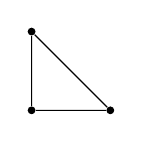
\begin{tikzpicture}
      \begin{scope}[every node/.style={inner sep=1pt, fill=black, circle}]

        \node (A) at (0,0) {};
        \node (B) at (1,0) {};
        \node (C) at (0,1) {};
        \draw (A) -- (B) -- (C) -- (A);
      \end{scope}
    \end{tikzpicture}
  \end{center}
\end{nthm}

\begin{proof}
  Form a tripartite graph with vertex sets $X=Y=[n]$, $Z=[2n]$, and edges:
  \begin{itemize}
    \item Join $x \in X$ to $y \in Y$ if $(x,y) \in A$.
    \item Join $x \in X$ to $z \in Z$ if $(x,z-x) \in A$.
    \item Join $y \in Y$ to $z \in Z$ if $(z-y,y) \in A$.
  \end{itemize}
  If $(x,y,z)$ is triangle, then, writing $d  = z-x-y$, we have
  \begin{align*}
    (x,y) \in A \quad (x,z-x) = (x,y+d) \in A \quad (z-y,y) = (x+d,y) \in A.
  \end{align*}
  So if $A$ contains no corners, then the only triangles are `degenerate' triangles where $x+y=z$, so $d=0$.
  So the number of triangles is at most $\delta n^2$.

  But the degenerate triangles are edge-disjoint, since any two of $x,y,z$ determine the third if $x+y=z$.
  So the number of edges you have to remove to get one of all triangles is at least $\delta n^2$.
  So the number of triangles is exactly $\delta n^2 = o(n^3)$.
  For sufficiently large $n$, this contradicts  the triangle removal lemma.
\end{proof}
%picture of roth's theorem

\clearpage
\section{The Polynomial Method}
On the example sheet, we proved Roth's theorem in $\mathbb{F}_3^n$, with a bound $\frac{C}{n}$.
This was beaten massively by a bound $c^n$, and we present the proof now.

\begin{defi}[Slice rank]
Let $X$ be a finite set and let $f: X^3 \to \mathbb{F}$ for some field $\mathbb{F}$.
The \named{slice rank} of $f$ is the smallest $k$ such that there are functions $u_1, \dotsc, u_k: X \to \mathbb{F}$, $v_1, \dotsc, v_k: X^2 \to \mathbb{F}$, $k_1,k_2$ such that
\begin{equation*}
  f(x,y,z) = \sum_{i=1}^{k_1} u_i(x) v_i(y,z) + \sum_{i={k+1}}^{k_2} u_i(y) v_i(x,z) + \sum_{i=k_2+1}^k u_i(z) v_i(x,y).
\end{equation*}
\end{defi}
\begin{nlemma}\label{lem:4.1}
  Let $X$ be a finite set, let $A \subset X$ and let $f: X^3 \to \mathbb{F}$ be a function such that for $x,y,z \in A$, $f(x,y,z) \neq 0$ iff $x=y=z \in A$. Then $f$ has \hyperlink{def:slicerank}{slice rank} $|A|$.
\end{nlemma}
\begin{proof}
  We can write $f(x,y,z)$ as
  \begin{equation*}
    \sum_{a \in \Lambda} \lambda_a \delta_a(x) \delta_a(y) \delta_a(z)
  \end{equation*}
  so the slice rank is at most $|A|$.
  Now suppose that
  \begin{equation*}
    f(x,y,z) = \sum_{i=1}^k{k_1} u_i(x) v_i(y,z) + \sum_{i=k_1+1}^{k_2} u_i(y) v_i(x,z) + \sum_{i=k_2+1}^{k} u_i(z) v_i(x,y).
  \end{equation*}
  Let $V$ be the subspace of $\mathbb{F}^*$ that consists of functions orthogonal to all of $u_1, \dotsc, u_{k_1}$.
  That is, $h \in V$ iff
  \begin{equation*}
    \sum_x h(x) u_i(x) = 0
  \end{equation*}
  for all $i \leq k_1$.
  Then $V$ has codimension at most $k_1$, it follows that $V$ contains some function $h$ that vanishes at most $k_1$ times.

  To see this, form an $m \times n$ matrix whose rows are a basis for $V$ (so $m \geq n-k_1$). Put the matrix into reduced row echelon form.
  Add up the rows to get the desired function.
  Now define $g: X^2 \to \mathbb{F}$ by
  \begin{equation*}
    g(y,z) = \sum_x f(x,y,z) h(x).
  \end{equation*}
  Then $g(y,z) \neq 0$ iff $y=z \in A$ and $h(y) \neq 0$.
  This holds at least $|A|-k_1$ times,  so $g$ has rank $\geq |A| - k_1$.

  But also, $g(y,z)$ has a formula of the formula of the form
  \begin{equation*}
    \sum_{i=k_1+1}^{k_2} u_i(y) w_i(z) + \sum_{k_2+1}^k u_i(z) w_i(y)
  \end{equation*}
  for some functions $w_i$ (if $k_1 < i \leq k_2$ then $w_i(z) = \sum_x u_i(x,z) h(x)$).
  Therefore, $g$ has rank at most $k-k_1$.
  Therefore, $|A| \leq k$.
\end{proof}
Let $F(n)$ be the number of $\{0,1,2\}$ sequences of length $n$ that at up to at most $\frac{2n}{3}$.
\begin{nlemma}
  Let $A$ be a subset of $\mathbb{F}_3^n$ such that if $x,y,z \in A$ and $x+y+z=0$ then $x=y=z$.
  Then $|A| \leq 3 F(n)$.
\end{nlemma}
\begin{proof}
  The function
  \begin{equation*}
    \sum_{a \in A} \delta_a(x) \delta_a(y) \delta_a(z)
  \end{equation*}
  on $A^3$ can be expressed by the formula
  \begin{equation*}
    f(x,y,z) = \sum_{i=1}^n (1-(x_i+y_i+z_i)^2).
  \end{equation*}
  This is a polynomial in $x_1, \dotsc, x_n, y_1, \dotsc, y_n, z_1, \dotsc, z_n$ with each $x_i,y_i,z_i$ occurring with degree $0,1$ or $2$.
  Also, it has total degree $2n$. It is therefore a linear combination of monomials, and in each one, either $x$ variables or $y$ variables or $z$ variables occur with total degree at most $\frac{2n}{3}$.
  Partition the monomials into three sets accordingly.

  It follows that we can write
  \begin{equation*}
    \sum_{a \in A} \delta_a(x) \delta_a(y) \delta_a(z)
  \end{equation*}
  as
  \begin{equation*}
    \sum_{i=1}^{m_1} u_i(x) v_i(y,z) + \sum_{i=m_1+1}{m_2} u_i(y) v_i(x,z) + \sum_{i=m_2+1}^m u_i(z) v_i(x,y)
  \end{equation*}
  where the $u_i$ are monomials of total degree at most $\frac{2n}{3}$ and the $v_i$ are polynomials (in $2n$ variables).
  The number of monomials in $x_1, \dotsc, x_n$ such that each $x_i$ occurs with degree $0,1$ or $2$ and the total degree is $\leq \frac{2n}{3}$ is $F(n)$ so $|A| \leq 3 F(n)$ by \cref{lem:4.1}.
\end{proof}
\begin{nlemma}\label{lem:4.3}
  \begin{equation*}
    F(n) \leq e^{-\frac{n}{12}} \cdot 3^n.
  \end{equation*}
\end{nlemma}
\begin{proof}
  Let $x$ be a random sequence in $\{0,1,2\}^n$ and let $X_1, \dotsc, X_n$ be independent random variables uniformly distributed in $\{-1,0,1\}$.
  Then
  \begin{align*}
    \mathbb{P}\left[\sum x_i \leq \frac{2n}{3}\right] &= \mathbb{P}\left[\sum_{i=1}^n X_i \geq \frac{n}{3}\right] \\
                                           &= \mathbb{P}\left[e^{\lambda \sum_{i=1}^n X_i} \geq e^{\lambda \frac{n}{3}}\right] \\
                                           &\leq e^{-\frac{\lambda n}{3}} \mathbb{E} e^{\lambda \sum_{i=1}^n X_i} \\
                                           &= e^{-\frac{\lambda n}{3}} \prod_{i=1}^n (\mathbb{E} e^{\lambda x_i}) \\
                                           &= e^{-\frac{\lambda n}{3}} \left(\frac{1 + e^\lambda + e^{-\lambda}}{3}\right)^n.
  \end{align*}
  But
  \begin{align*}
    \frac{1+e^\lambda + e^{-\lambda}}{3} &= 1 + \frac{2}{3} \frac{\lambda^2}{2!} + \frac{2}{3} \frac{\lambda^4}{4!} + \dotsb \\
                                         &= 1 + \frac{\lambda^2}{3} + \left(\frac{\lambda^2}{3}\right)^2 \frac{1}{2!} + \left(\frac{\lambda^2}{3}\right)^3 \frac{1}{3!} + \dotsb \\
                                         &= e^{\frac{\lambda^2}{3}}
  \end{align*}
  So the probability is at most $e^{-\frac{\lambda n}{3} + \frac{\lambda^2 n}{3}}$.
  By choosing $\lambda = \frac{1}{2}$ gives an upper bound of $e^{-\frac{n}{12}}$.
\end{proof}
\begin{nthm}
  Let $A \subset \mathbb{F}_3^n$ contain no nontrivial solutions to $x+y+z=0$. Then $|A| \leq e^{-\frac{n}{12}} \cdot 3^n$.
\end{nthm}

Our next target is the finite-fields Kakeya theorem of Zeev Dvir.
\begin{nlemma}\label{lem:4.5}
  Let $A \subset \mathbb{F}_p^N$.
  If $|A| < \binom{n + d}{n}$ then there exists a non-zero polynomial of degree at most $d$ that vanishes everywhere on $A$.
\end{nlemma}
\begin{proof}
  A polynomial $P$ of degree $\leq d$ has a formula
  \begin{equation*}
    P(x) = \sum_{|E| \leq d} \lambda_E \prod_{i \in E} x_i
  \end{equation*}
  where $E$ is a multiset. So for $P$ to vanish on $A$, we need
  \begin{equation*}
    \sum_{|E| \leq d} \lambda_E \prod_{i \in E} a_i
  \end{equation*}
  to be zero for every $a \in A$.
  This gives $|A|$ linear equations that the coefficients $\lambda_E$ must solve.
  Given a subset $m_1 < m_2 < \dotsb < m_n$ of $[n+d]$, we can define a monomial $x_1^{r_1} \dotsm x_n^{r_n}$ of degree $\leq d$ by setting $r_1 = m_1 - 1, r_i = m_i - m_{i-1} - 1$ for $i > 1$, since $r_1 + \dotsb + r_n = m_n - n \leq d$.
  Moreover, this is a bijection.
  So the number of monomials is $\binom{n+d}{n}$.
  So if $|A| < \binom{n+d}{n}$ we get a non-trivial choice for the $\lambda_t$.
\end{proof}

\begin{nlemma}
  Let $P$ be a polynomial of degree $<p$ that vanishes everywhere on $\mathbb{F}_p^n$. Then $P$ is the zero polynomial.
\end{nlemma}
\begin{proof}
  If $n=1$, then $P$ has $p$ roots and degree $<p$, so it must be the zero polynomial.
  If $n > 1$, then we can write
  \begin{equation*}
    P(x) = P_0(x_2, \dotsc, x_n) + x_1 P_1(x_2, \dotsc, x_n) + x_1^2 P_2(x_2, \dotsc, x_n)+ \dotsb + x_1^{p-1} P_{p-1}(x_2, \dotsc, x_n).
  \end{equation*}
  For every choice of $x_2, \dotsc, x_n$, the RHS vanishes for all $x_1$ so is the zero polynomial and therefore all the $P_i$ vanish everywhere. Hence by induction, the $P_i$ are all the zero polynomial.
\end{proof}
\begin{thm}
  Let $A \subset \mathbb{F}_p^n$ be a set and suppose that for every $\vec{d} \neq 0$ there exists $\vec{a}$ such that the set
  \begin{equation*}
    \set{\vec{a} + \lambda \vec{d} | \lambda \in \mathbb{F}_p} \subset A.
  \end{equation*}
  Then $|A| \geq \frac{p^n}{n!}$.
\end{thm}
\begin{proof}
  By \cref{lem:4.5}, if $|A| < \binom{n+p-1}{n}$ then there is a non-zero polynomial $Q$ of degree $<p$ that vanishes on $A$.
  Let $\deg Q = m$ and let $Q_m$ be the homogeneous polynomial consisting of the degree $m$ terms of $Q$.

  For each $\vec{d} \neq 0$ we know that $Q$ vanishes on some line $\{\vec{a} + \lambda \vec{d}\}$.
  But $Q$ restricted to $\{\vec{a} + \lambda \vec{d}\}$ is a polynomial in $\lambda$ of degree $<p$, so it is the zero polynomial.
  The degree-$m$ coefficient of this restriction is $Q_m(\vec{d})$ (since `to get $\lambda^m$ we must choose $\lambda d_i$ from each bracket').
  So $Q_m(\vec{d}) = 0$ for every $\vec{d} = 0$. Trivially $Q_m(\vec{0}) = 0$ too. So $Q_m$ is the zero polynomial.
  Therefore
  \begin{equation*}
    |A| \geq \binom{n+p-1}{n} = \frac{(n+p-1)(n+p-2) \dotsm p}{n!} \geq \frac{p^n}{n!}. \qedhere
  \end{equation*}
\end{proof}

\section{A taste of higher-order Fourier analysis}
Let $k \geq 1$. Given finite sets $X_1, \dotsc, X_k$ and a function $f: X_1 \times \dotsb \times X_k \to \mathbb{C}$, we define the $k$-dimensional box-norm $\|f\|_\square$ of $f$ by the formula
\begin{equation*}
  \|f\|_\square^{2^k} = \E_{\substack{x_1^0, \dotsc, x_k^0\\x_1^1, \dotsc, x_k^1}} \prod_{\epsilon \in \{0,1\}^k} C^{|\epsilon|} f(x_1^{\epsilon_1}, \dotsc, x_k^{\epsilon_k})
\end{equation*}
where $|\epsilon| = \epsilon_1 + \dots + \epsilon_k$ and $C$ is complex conjugation.
It can be shown that this is a norm.

\subsection{The \texorpdfstring{$U^k$}{U} norms}
Let $G$ be an Abelian group and let $f: G \to \mathbb{C}$.  Then we define $\|f\|_{U^2}$ by the formula
\begin{align*}
  \|f\|_{U^2}^4 &= \E_{x,a,b} f(x) \overline{f(x+a)} \overline{f(x+b)} f(x+a+b) \\
                &= \E_{x+y = z+w} f(x) f(y) \overline{f(z)} \overline{f(w)} \\
                &= \langle f * f, f * f \rangle = \|f \times f\|_2^2 = \|\hat{f}^2\|^2 = \sum_{\chi} |\hat{f}(\chi)|^4
\end{align*}
We also define $\|r\|_{U^3}$ by the formula
\begin{equation*}
  \|f\|_{U^3}^8 = \E_{x,a,b,c} f(x) \overline{f(x-a)} \overline{f(x-b)} f(x-a-b) \overline{f(c)} f(x-a-c) f(x-b-c) \overline{f(x-a-b-c)}.
\end{equation*}
If $F(x,y,z) = f(x+y+z)$, then $\|f\|_{U^3} = \|F\|_\square$. (Exercise).
In fact, if $r,s,t$ are coprime to the order of $G$, then the same is true of $F(x,y,z) = f(rx+sy+tz)$.
The 3d box norm satisfies the box-norm inequality (from sheet 3)
\begin{equation*}
  \abs{\E_{x,y,z} f(x,y,z) u(x,y) v(x,z) w(y,z)} \leq \|f\|_\square \|u\|_\infty \|v\|_\infty \|w\|_\infty.
\end{equation*}
\begin{nlemma}
  Let $G$ be a finite Abelian group with order not divisible by 2 or 3, and let $f_1, f_2, f_3, f_4: G \to \mathbb{C}$. Then
  \begin{equation*}
    \abs{\E_{x,d} f_1(x) f_2(x+d) f_3(x+2d) f_4(x+3d)} \leq \|f_1\|_{U^3} \|f_2\|_\infty \|f_3\|_\infty \|f_4\|_\infty.
  \end{equation*}
\end{nlemma}
\begin{proof}
  \begin{align*}
    \text{LHS} &= |\E_{x,y,z} f_1(-3x-2y-z) f_2(-2x-y) f_3(-x+z) f_4(y+2z)| \\
               &\leq \|f_1\|_{U^3} \|f_2\|_\infty \|f_3\|_\infty \|f_4\|_\infty
  \end{align*}
  by the previous remarks.
\end{proof}
\begin{ncor}
  Let $A,B$ be subsets of a finite Abelian group $G$ with order coprime to 2 and 3. Let $A$ have density $\alpha$, $B$ have density $\beta$. Suppose that $f = A-\alpha$ has the property that $\|f\|_{U^3} \leq c$.
  Then $|\E_{x,d} A(x) A(x+d) B(x+2d) B(x+3d) - \alpha^2 \beta^2| \leq 2c$.
\end{ncor}
\begin{proof}
  Let $B = \beta + g$. Then
  \begin{align*}
    \E_{x,d} A(x) A(x+d) B(x+2d) B(x+3d) = \E_{x,d} (\alpha+f(x)) (\alpha + f(x+d)) (\beta+g(x+2d))(\beta + g(x+3d)).
  \end{align*}
  This splits into 16 terms, one of which is $\alpha^2 \beta^2$.
  Of the remaining terms, we have a contribution of
  \begin{equation*}
    \E_{x,d} f(x) A(x+d) B(x+2d) B(x+3d)
  \end{equation*}
  from the terms where we pick $f(x)$ from the first bracket.
  By lemma 1, this is at most $c$. If we choose $\alpha$ from the first bracket and $f(x+d)$ from the second, we get a contribution $\alpha \E_{x,d} f(x+d) B(x+2d) B(x+3d) = \alpha \E_{x,d} f(x) B(x+d) B(x+2d)$, which also has magnitude at most $c$. All other contributions are zero.
\end{proof}

If $\|f\|_{U^3}$ is small, then $A$ contains roughly the right number of 4APs.
What happens if $\|f\|_{U^3}$ is large?
\begin{defi}
  Let $G$ be a finite abelian group, $f: G \to \mathbb{C}$, $a \in G$.
  Write $\partial_a f$ for the function $\partial_a f(x) = f(x) \overline{f(x-a)}$.
\end{defi}
This is in some sense a multiplicative discrete derivative: if $f(x) = \omega^{\phi(x)}$ then $\partial_a f(x) = \omega^{\phi(x) - \phi(x-a)}$.

Observe that
\begin{align*}
  \|f\|^8_{U^3} &= \E_{x,a,b,c} f(x) \overline{f(x-a)} \dotsm \overline{f(x-a-b-c)}  \\
                &= \E_{x,a,b,c} \partial_a f(x) \overline{\partial_a f(x-b)} \overline{\partial_a f(x-c)} \partial_a(f-b-c) \\
                &= \E_a \|\partial_a f\|^4_{U^2} \\
                &= \E_a \sum_r |\widehat{\partial_a f}(r)|^4 \leq \E_a \max_{r} \abs{\widehat{\partial_a f}(r)}^2 \sum_r |\widehat{\partial_a f}(r)|^2.
\end{align*}
So if $\|f\|^8_{U^3} \geq c$, $\E_a \max_r \abs{\widehat{\partial_a f}(r)}^2 \geq c$.
\begin{align*}
  &\implies \exists B \text{ such that } |B| \geq \frac{c}{2} |G| \text{ and } \max_r \abs{\widehat{\partial_a f}(r)}^2 \geq \frac{c}{2} \text{ for every } a \in B. \\
  &\implies \exists B, \varphi: B \to \hat{G} \text{ such that } \E_a B(a) \abs{\widehat{\partial_a f}(\phi(a))}^2 \geq \frac{c^2}{4}.
\end{align*}
So
\begin{align*}
  \frac{c^2}{4} &\leq \E_a B(a) \abs{\widehat{\partial_a f}(\phi(a))}^2 \\
                &= \E_a B(a) \E_{x,y} f(x) \overline{f(x-a)} \overline{f(y)} f(y-a) \omega^{-\phi(a) \cdot (x-y)} \\
                &= \E_{b,x,z} f(x) \overline{f(z)} \overline{f(x-b)} f(z-b) \omega^{-\phi(x-z) \cdot b)} B(x-z) \\
                &\leq \E_b \|F_b\|_\square \qquad \text{where } F_b(x,y) = \omega^{-b \cdot \phi(x-z)} B(x-z) \\
                &\leq (\E_b \|F_b\|_\square^4)^{\frac{1}{4}} \\
                &= \left(\E_b \E_{\substack{x_1,x_2 \\ z_1,z_2}} B(x_1-z_1) B(x_1-z_2) B(x_2-z_1) B(x_2-z_2) \omega^{-b \cdot (\phi(x_1-z_1) - \phi(x_1-z_2) - \phi(x_2-z_1) + \phi(x_2-z_2)})\right)^\frac{1}{4} \\
                &= \left(\E_{t+u=v+w} B(t) B(v) B(w) B(u) \underbrace{\E_b \omega^{-b \cdot (\phi(t) + \phi(u) - \phi(v) + \phi(w))}}_{=\mathbbm{1}_{\phi(t) + \phi(u) = \phi(v) + \phi(w)}}\right)^\frac{1}{4} \\
                &= \mathbb{P}_{t+u=v+w} \left[t,u,v,w \in B \text{ and } \phi(t) + \phi(u) = \phi(v) + \phi(w)\right].
\end{align*}
Equivalently, if $\Gamma = \set{(x,\phi(x)) : x \in B}$ is the graph of $\phi$, then $\Gamma$ contains at least $\frac{c^8}{256} |\Gamma|^3$ additive quadruples.
So by BSG, $\Gamma$ has a large subset $\Gamma'$ such that $|\Gamma' - \Gamma'| \leq C |\Gamma'|$.
Then by the proof of Freiman's theorem, $2 \Gamma' - 2G'$ contains a subset isomorphic to a low dimensional Bohr set $B$.
But low dimensional Bohr sets contain longish arithmetic APs.
So $2\Gamma' - 2\Gamma'$ contains a fairly long AP $P$.

Let $X \subset \Gamma'$ be maximal such that sets $x+P$, $x \in X$ are disjoint.
Then $|X| |P| = |X+P| \leq \abs{3\Gamma' - 2 \Gamma'} \leq C^5 |\Gamma'|$.
Also, $\Gamma' \subset X + P - P$ by maximality.
So $\Gamma'$ is contained in the union of $\leq \frac{C^5 |\Gamma'|}{|P|}$ translates of $P$.
So one of these translates contains at least $\frac{|P|}{C^5}$ points of $\Gamma'$.

Now let's oversimplify and assume that $B = \mathbb{Z}_N$ and $\phi(x) = 2 \lambda x$ for every $x$.
Then
\begin{align*}
  c \leq \E_a |\widehat{\partial_a f} (2 \lambda a)|^2 = \E_{a,b} f(x) \overline{f(x-a)} \overline{f(x-b)} f(x-a-b) \omega^{-2\lambda a b }
\end{align*}
But $2ab = x^2 - (x-a)^2 - (x-b)^2 + (x-a-b)^2$, so the right hand side is
\begin{align*}
  &= \E_{a,x,b} g(x) \overline{g(x-a)} \overline{g(x-b)} g(x-a-b) \\
  \shortintertext{where $g(x) = f(x) \omega^{\lambda x^2}$.}
  &= \|g\|_{U^2}^4 = \sum_r \abs{\hat{g}(r)}^4 \leq \max_r |\hat{g}(r)|^2
\end{align*}
So $\exists r$ such that $c^\frac{1}{2} \leq |\hat{g}(r)| = \abs{\E_x f(x) \omega^{\lambda x^2 - r x}}$.

Claim: for all $r$, we can find $d \leq m$ such that $\omega^{r d^2}$ is close to 1.

Divide the circle into arcs of length $\leq \epsilon$. By van der Waerden's theorem we can find $x-d, x, x+d$ such that $\frac{(x-d)^2}{2}, \frac{x^2}{2}, \frac{(x+d)^2}{2}$ all lie in the same interval.
But then $d^2 = \frac{(x-d)^2}{2} - 2 \cdot \frac{x^2}{2} + \frac{(x+d)^2}{2}$ is small, so $\omega^{d^2} \approx 1$.
\end{document}
